% !TeX program = xelatex
\documentclass[12pt,a4paper]{article}
\usepackage{fontspec}
\usepackage{polyglossia}
\setdefaultlanguage{russian}
\setmainfont{Times New Roman}
\setmonofont{Courier New}
\newfontfamily\cyrillicfonttt[Script=Default]{Courier New}
\usepackage{amsmath,amssymb}
\usepackage[margin=2cm]{geometry}
\usepackage{graphicx,longtable,array}
\PassOptionsToPackage{obeyspaces}{url}
\usepackage[unicode,hidelinks]{hyperref}
\setlength{\parindent}{0pt}
\setlength{\parskip}{6pt}
\setlength{\emergencystretch}{3em}
\AtBeginEnvironment{verbatim}{\small}
\renewcommand{\arraystretch}{1.25}
\newcommand{\micro}[1]{\subsection{#1}}
\newcommand{\taskhead}[1]{\par\textbf{#1}\par}

\usepackage{xcolor}

\newsavebox{\nbbox}
\newenvironment{notabene}
  {\par\medskip
   \begin{lrbox}{\nbbox}%
   \begin{minipage}{\dimexpr\linewidth-20pt\relax}
   {\fontsize{13}{16}\selectfont\bfseries
    \color{black!85}NB\par}
   \vspace{4pt}
   \noindent\ignorespaces}
  {\par\end{minipage}%
   \end{lrbox}%
   \noindent
   \begingroup
   \setlength{\fboxsep}{10pt}%
   \colorbox{blue!5}{\usebox{\nbbox}}%
   \endgroup
   \par\medskip}

\usepackage{listings}
\usepackage{xcolor}

% Сохранять ASCII-дефис U+002D при копировании кода из PDF.
\lstset{literate={-}{{\char45}}1}

\lstdefinestyle{commands}{
  basicstyle=\ttfamily\small,
  backgroundcolor=\color{gray!10},
  frame=single,
  framerule=0pt,
  framesep=8pt,
  framexleftmargin=6pt,
  xleftmargin=14pt,
  xrightmargin=8pt,
  breaklines=true,
  columns=fullflexible,
  keepspaces=true,
  showstringspaces=false
}

\usepackage{xparse}
\usepackage{xcolor}

\NewDocumentCommand{\func}{v}{%
  \colorbox{gray!15}{\texttt{#1}}%
}

\begin{document}
\sloppy
\begin{center}
{\LARGE\bfseries Лабораторная работа по линейной алгебре \\ (1 семестр)\par}
\vspace{0.4em}
{\large Системы линейных уравнений, кривые второго порядка\par
и векторное представление текстов\par}
\end{center}

\section*{Описание лабораторной работы}
Цель работы --- применить методы линейной алгебры к вычислению определителей,
решению систем линейных уравнений, смене базиса, приведению кривых второго порядка
к каноническому виду и векторному представлению текстов. Работа объединяет три тематических раздела:
\begin{enumerate}
\item Вычисление определителей, решение СЛАУ и нахождение координат вектора в новом базисе.
\item Приведение кривых второго порядка к каноническому виду.
\item Поиск наиболее релевантных документов по запросу с использованием TF-IDF (Term Frequency-Inverse Document Frequency).
\end{enumerate}

{
Все три раздела объединяет идея представления объектов с помощью векторов и координат. 
Выбор представления помогает упростить задачу и заметить, какие свойства сохраняются при преобразованиях координат.
}

Для выполнения использовать базовые сведения о матрицах, векторах и Python.
Необходимые дополнительные теоретические сведения приведены непосредственно перед соответствующими разделами.
Входные данные для реализации алгоритмов и аналитических вычислений приведены в приложении А.

\section*{Порядок выполнения лабораторной работы}
\begin{enumerate}

\item Преподаватель назначает номер варианта $k$. 
Данный номер используется во всех таблицах и списках вариантов приложения А. 
Выполнению подлежат задания только своего варианта.
\item Далее начинается подготовка программного окружения. 
Этапы подготовки описаны в разделе 0.
\item В разделе 1 вычислить определитель, решить СЛАУ и найти координаты
вектора в другом базисе. Вычисления выполнить аналитически, затем реализовать
функции и сравнить результаты.
\item В разделе 2 аналитически выполнить приведение одной кривой второго порядка к каноническому виду.
\newpage
\item В разделе 3 последовательно реализовать обработку текста, TF, IDF,
TF-IDF, косинусную близость и ранжирование. Для каждой задачи данного раздела
сопоставить результаты аналитических вычислений своего варианта с результатами выполнения реализованных функций.
\item Результаты всей работы оформляются в виде отчёта в LaTeX и собранного PDF. К отчёту прилагаются исходный код,
исходники отчёта, теоретические выкладки, вычисления невязок, абсолютных и относительных ошибок и изображения согласно требованиям раздела 4.
\end{enumerate}

\section*{Требования к выполнению}
Определения абсолютной и относительной ошибок, невязки, а также правила сравнения
аналитических и программных результатов приведены в конце раздела
«Требования к отчёту и составу сдаваемых материалов».

\begin{itemize}

\item Все файлы, необходимые для выполнения лабораторной работы, размещены в репозитории GitHub: \url{https://github.com/xhiggs/linear_algebra_lab_1_sem}. 
Перед началом работы следует скачать репозиторий и перейти в папку, в которой расположены все файлы, необходимые для выполнения работы.
\item Работа выполняется в командах по 2--4 человека. Сохранить заданные в \func{solution.py} имена функций,
состав и порядок аргументов, а также форматы возвращаемых результатов. Входные данные изменять нельзя.
\item В разделе 1 использовать списки, циклы, арифметику и собственные функции.
Нельзя использовать готовые решатели, \func{numpy.linalg}, SymPy, вычисление
обратной матрицы или рекурсивный перебор миноров.
\item В разделе 3 использовать NumPy для операций над массивами.
Нельзя использовать готовые TF-IDF-векторизаторы и поисковые реализации, включая
соответствующие средства sklearn. 
Не допускается подмена вычислений заранее заданными ответами или промежуточными числовыми результатами для конкретного варианта.
\item Аналитические вычисления представляются как последовательность формул с пояснениями.
Дроби и корни записываются в точном виде; для логарифмов дополнительно приводятся
приближения не менее чем с шестью знаками после запятой.
\item Каждая программируемая задача соответствующего раздела завершается запуском указанной проверки.
Общие тесты проверяют алгоритм; дополнительно необходимо вызвать функции на данных
своего варианта. Результат тестов не заменяет индивидуальное сравнение.
\item {Использование ИИ для написания отдельных блоков не запрещено. 
Однако, помощь искусственного интеллекта не заменяет необходимость понимать, 
что происходит во всех блоках алгоритмов, реализованных в файле \func{solution.py}.
Пример написания кода с помощью ИИ приведен в разделе 3 в примере для первой задачи 3.1.}
\end{itemize}

\newpage

\setcounter{section}{-1}
\section{Подготовка рабочего окружения}
\taskhead{Файлы для выполнения задач данного раздела}
\begin{itemize}
\item \func{requirements.txt} --- список библиотек для установки в локальное окружение.
\item \func{run.py} --- запуск команды \func{--list} для проверки доступности тестов.
\item \func{report.tex} --- создаваемый студентом файл отчёта, в котором указываются сведения об окружении.
\end{itemize}

\taskhead{Описание и порядок выполнения}
Для работы требуется Python версии 3.10 или новее. Рабочей папкой является папка лабораторной,
содержащая \func{solution.py}, \func{run.py} и \func{requirements.txt}.
Все команды Python выполняются из этой папки.
\begin{longtable}{p{0.32\textwidth}p{0.61\textwidth}}
\textbf{Файл} & \textbf{Назначение}\\\hline
\func{solution.py} & Заготовки математических функций.\\
\func{run.py}, \func{tests/} & Поэтапные проверки и диагностический вывод.\\
\func{requirements.txt} & Зависимости Python.\\
\func{data/documents.json} & Корпус английских текстов для поиска.\\
\func{demo_text.py} & Готовый запуск поиска на корпусе.\\
\func{main.tex} & Настоящее условие; отчёт оформляется в отдельном файле.\\
\end{longtable}

\taskhead{Создание окружения}
Для macOS и Linux используются следующие команды:
\begin{lstlisting}[style=commands]
python -m venv .venv
source .venv/bin/activate
pip install -r requirements.txt
\end{lstlisting}
Для Windows PowerShell используются следующие команды:
\begin{lstlisting}[style=commands]
py -m venv .venv
.\.venv\Scripts\Activate.ps1
python -m pip install -r requirements.txt
\end{lstlisting}
Если PowerShell запрещает запуск сценария активации, выполнить команды
через интерпретатор окружения:
\begin{lstlisting}[style=commands]
.\.venv\Scripts\python.exe -m pip install -r requirements.txt
.\.venv\Scripts\python.exe run.py --list
\end{lstlisting}
В остальных командах при необходимости заменить \func{python}
на этот путь. В командной строке Windows cmd для активации окружения использовать команду
\begin{lstlisting}[style=commands]
  .\.venv\Scripts\activate.bat
\end{lstlisting}

\newpage

\taskhead{Проверка установки библиотек и окружения}

Для проверки корректности установки соответствующих библиотек для Python запустить в консоли команду:

\begin{lstlisting}[style=commands]
python -c "import numpy, matplotlib; print(numpy.__version__)"
python run.py --list
\end{lstlisting}

\underline{Ожидаемый результат} --- версия NumPy и перечень доступных проверок без ошибок импорта.

При запуске тестов без реализации соответствующих функций ожидаемо получить ошибку \func{NotImplementedError}. После установки зависимостей тесты работают
без интернета. Перед началом каждой новой рабочей сессии активировать окружение в терминале.

Для macOS и Linux:

\begin{lstlisting}[style=commands]
source .venv/bin/activate
\end{lstlisting}

Для Windows PowerShell:

\begin{lstlisting}[style=commands]
.\.venv\Scripts\Activate.ps1
\end{lstlisting}

Для отчёта также установить дистрибутив LaTeX с XeLaTeX. Cобрать отдельный
файл \func{report.tex} командой \func{xelatex report.tex}; при наличии
\func{latexmk} использовать \func{latexmk -xelatex report.tex}.


\begin{notabene}
Для автоматической нумерации ссылок и оглавления в LaTeX выполнить сборку повторно.
В macOS при отсутствии команд в PATH использовать префикс
\func{/Library/TeX/texbin/}.
\end{notabene}

\newpage

\section{Определители, СЛАУ и координаты вектора}
\taskhead{Файлы для выполнения задач данного раздела}
\begin{itemize}
\item \func{solution.py} --- реализация функций \func{determinant}, \func{solve_cramer} и \func{change_coordinates}.
\item \func{run.py} --- запуск проверок \func{determinant}, \func{cramer} и \func{coordinates}.
\item \func{tests/} --- готовые проверки, необходимые для запуска тестов.
\item \func{variant_check.py} --- создаваемый студентом скрипт вызова своих функций на данных варианта и вывода результатов.
\item \func{report.tex} --- аналитические решения, программные результаты, абсолютные и относительные ошибки; для СЛАУ и смены базиса --- также невязки. Исходные данные приведены в приложениях А.1--А.3.
\end{itemize}

\taskhead{Описание}
Требуется реализовать три функции:
\begin{itemize}
\item \func{determinant} --- вычисление определителя;
\item \func{solve_cramer} --- решение СЛАУ методом Крамера;
\item \func{change_coordinates} --- нахождение координат вектора в новом базисе.
\end{itemize}
Изменения вносятся в \func{solution.py}.
Проверки запускаются из папки лабораторной работы соответствующими командами.
Полный перечень проверок доступен по команде 

\begin{lstlisting}[style=commands]
python run.py --list
\end{lstlisting}

\taskhead{Правила выполнения}
Выполнить задачи данного раздела 1.1--1.3 последовательно. Для каждой задачи указать:

\begin{itemize}
  \item Исходные данные своего варианта из приложения А
  \item Аналитическое решение с пояснениями
  \item Реализацию функции в \func{solution.py}
  \item Запуск тестов соответствующей функции
  \item Вызов функции на своих данных и вывод результата
  \item Сравнение аналитического и программного результатов, вычисление абсолютной и относительной ошибок, а также невязки для СЛАУ и смены базиса
\end{itemize}

\micro{Вычисление определителя}
\taskhead{Теория}

Определитель --- число, сопоставленное квадратной матрице. Ненулевой
определитель матрицы коэффициентов обеспечивает единственность решения
квадратной СЛАУ. 

Для матрицы размера $1\times1$ принимается $\det[a]=a$, а для $2\times2$:
\[
\det\begin{pmatrix}a&b\\c&d\end{pmatrix}=ad-bc.
\]
Для общего размера используются элементарные преобразования строк: элементы под главной
диагональю последовательно обращаются в ноль. Обозначение $R_i$ соответствует
строке с номером $i$. В аналитических примерах строки нумеруются с единицы,
а в Python --- с нуля. При вычислении определителя используются свойства:
\begin{itemize}
\item $R_i\leftrightarrow R_j$: перестановка двух строк меняет знак определителя;
\item $R_i\gets R_i+\alpha R_j$, $i\ne j$: прибавление кратной другой строки
сохраняет определитель;
\item определитель верхнетреугольной матрицы равен произведению диагональных элементов.
\end{itemize}
Верхнетреугольная матрица имеет нули ниже главной диагонали. Одних
перестановок строк в общем случае недостаточно: они позволяют выбрать
ненулевой ведущий элемент, а вычитание кратных строк создаёт нужные нули.
При умножении всей строки на число $\alpha$ определитель также умножается
на $\alpha$. Поэтому в рассматриваемом алгоритме ведущая строка не нормируется.

После $m$ перестановок строк и исключения элементов получается матрица $U$.
Исходный определитель восстанавливается по формуле
\[
\det A=(-1)^m u_{11}u_{22}\cdots u_{nn},
\]

где $u_{ii}$ --- элементы главной диагонали полученной
верхнетреугольной матрицы $U$, а $m$ --- число перестановок строк.

\taskhead{Порядок выполнения}
\begin{enumerate}
  \item Взять матрицу $A_k$ из приложения А.1.
  \item Вычислить её определитель аналитически.
  Привести последовательность элементарных преобразований
  строк, указать число перестановок и произведение
  диагональных элементов полученной верхнетреугольной матрицы.
  \item Реализовать \func{determinant(matrix)} для квадратной матрицы
  порядка $n \geq 1$ путём приведения к верхнетреугольному виду
  с помощью элементарных преобразований строк.
  При вычислении определителя учитывать изменение знака
  при каждой перестановке строк.
  
  Допускаются перестановки строк и прибавление к одной строке
  другой строки, умноженной на число. Деление строки
  на ведущий элемент не выполнять.\\
  \item Проверить реализацию, выполнив команду:
  \begin{lstlisting}[style=commands]
python run.py unittest determinant\end{lstlisting}
  \item Вызвать функцию на матрице своего варианта.
  Сопоставить аналитический и программный результаты,
  вычислить абсолютную и относительную ошибки.
\end{enumerate}

\begin{notabene}
Проверять в коде ведущий элемент на точный ноль: малый ненулевой элемент
сам по себе не означает малый определитель. Например,
$\det\operatorname{diag}(10^{-12},10^{12})=1$.
\end{notabene}

\underline{Ожидаемый результат}: число $\det A_k$, совпадающее с аналитическим ответом,
абсолютная и относительная ошибки и успешные тесты размеров 1--12, перестановок и зависимых строк.
Сравнить результаты аналитического и программного вычислений, вычислить абсолютную и относительную ошибки.

\taskhead{Пример}
В простейшем случае матрицы размера $2\times 2$ нулевой первый элемент устраняется перестановкой:

\[
A=\begin{pmatrix}0&2\\3&4\end{pmatrix}
\xrightarrow{R_1\leftrightarrow R_2}
U=\begin{pmatrix}3&4\\0&2\end{pmatrix}.
\]

У матрицы $U$ определитель равен $3\cdot2=6$. Выполнена одна перестановка,
поэтому $\det A=-\det U=-6$. Прямая проверка: $0\cdot4-2\cdot3=-6$.

Рассмотрим матрицу размера $3\times 3$:
\[
A=\begin{pmatrix}0&2&1\\1&1&0\\2&0&1\end{pmatrix}.
\]
В первом столбце наибольший модуль имеет элемент 2 третьей строки.
После перестановки первой и третьей строк знак становится равным $-1$:
\[
A\xrightarrow{R_1\leftrightarrow R_3}
A^{(1)}=\begin{pmatrix}2&0&1\\1&1&0\\0&2&1\end{pmatrix}.
\]
Для второй строки множитель равен $\alpha=1/2$. Вычитание выполняется
для всех её элементов: $(1,1,0)-\tfrac12(2,0,1)=(0,1,-\tfrac12)$.
\[
A^{(1)}\xrightarrow{R_2\gets R_2-\frac12R_1}
A^{(2)}=\begin{pmatrix}2&0&1\\0&1&-\frac12\\0&2&1\end{pmatrix}.
\]

\newpage

В третьей строке первый элемент уже равен нулю. Теперь ведущий элемент
второго столбца выбирается только среди второй и третьей строк:
$|2|>|1|$. После их перестановки знак вновь равен $+1$:
\[
A^{(2)}\xrightarrow{R_2\leftrightarrow R_3}
A^{(3)}=\begin{pmatrix}2&0&1\\0&2&1\\0&1&-\frac12\end{pmatrix}.
\]
Остаётся вычесть из третьей строки половину второй:
\[
(0,1,-\tfrac12)-\tfrac12(0,2,1)=(0,0,-1),
\]
\[
A^{(3)}\xrightarrow{R_3\gets R_3-\frac12R_2}
U=\begin{pmatrix}2&0&1\\0&2&1\\0&0&-1\end{pmatrix}.
\]
Выполнены две перестановки. Прибавления кратных строк определитель не
изменили, поэтому
\[
\boxed{\det A=(-1)^2\cdot2\cdot2\cdot(-1)=-4}.
\]
Множитель $(-1)^2$ учитывает только количество перестановок, а отрицательный последний
элемент диагонали входит в произведение отдельно. Это разные источники знака.
Если на очередном шаге все доступные элементы столбца равны нулю,
получить ненулевой ведущий элемент перестановкой невозможно, и алгоритм
возвращает нулевой определитель.

\micro{Решение системы методом Крамера}
\taskhead{Теория}

Представление вектора в базисе также сводится к СЛАУ:
коэффициенты линейной комбинации базисных векторов являются искомыми
координатами.

Для системы $Ax=b$ при $\det A\ne0$ использовать формулу
\[
x_j=\frac{\det A_j}{\det A},
\]
где $A_j$ получена заменой столбца $j$ на $b$.
Невязка $r=Ax-b$ характеризует выполнение исходных уравнений найденным
решением. При точном решении $r=0$.

\taskhead{Порядок выполнения}

\begin{enumerate}
  \item Взять матрицу $B_k$ и вектор $b_k$ из приложения А.2.
  \item Решить систему $B_kx=b_k$ аналитически методом Крамера.
  Привести вычисление основного определителя, матрицы
  с заменёнными столбцами и их определители.
  Найти каждую неизвестную как отношение соответствующего
  заменённого определителя к основному.
  
  \newpage
  
  \item Реализовать \func{solve_cramer} для квадратной системы
  с ненулевым определителем, используя собственную функцию
  \func{determinant} из пункта 1.1.

  Основной определитель вычислить один раз.
  Для каждой неизвестной создать отдельную копию исходной
  матрицы и заменить соответствующий столбец вектором
  правой части. Исходные данные не изменять.
  При \func{abs(det(A)) <= tol} вызвать
  исключение \func{ValueError}.

  Не заменять метод Крамера непосредственным решением
  системы с помощью элементарных преобразований строк.
  Эти преобразования использовать только для вычисления
  определителей.
  \item Проверить реализацию, выполнив команду:
  \begin{lstlisting}[style=commands]
  python run.py unittest cramer\end{lstlisting}
  \item Вызвать функцию на данных своего варианта.
  Сопоставить аналитический и программный результаты,
  вычислить абсолютную и относительную ошибки.
  \item Подставить программно полученное решение $\widehat{x}$
  в исходную систему. Вычислить вектор невязки
  $r=B_k\widehat{x}-b_k$ и максимальный модуль его компонент.
\end{enumerate}

Во всех трёх задачах данного раздела использовать один и тот же
реализованный алгоритм вычисления определителя.

\underline{Ожидаемый результат}: вектор решения своего варианта, абсолютная и относительная ошибки
относительно аналитического решения, вектор невязки $r=A\widehat x-b$
и максимальный модуль его компонент, близкий к нулю.

\taskhead{Пример}

Для
\[
A=\begin{pmatrix}2&1\\1&-1\end{pmatrix},\quad
b=\begin{pmatrix}5\\1\end{pmatrix}
\]
заменяются именно столбцы, содержащие коэффициенты соответствующих неизвестных:
\[
A_1=\begin{pmatrix}5&1\\1&-1\end{pmatrix},\qquad
A_2=\begin{pmatrix}2&5\\1&1\end{pmatrix}.
\]
В $A_1$ заменён только первый столбец исходной матрицы $A$, в $A_2$ --- только второй.
Матрица $A_2$ не получается из $A_1$: каждая замена начинается с исходной матрицы.
\begin{align*}
\det A&=2\cdot(-1)-1\cdot1=-3,\\
\det A_1&=5\cdot(-1)-1\cdot1=-6,\\
\det A_2&=2\cdot1-5\cdot1=-3.
\end{align*}
Следовательно, $x=(-6)/(-3)=2$, $y=(-3)/(-3)=1$.
Проверка выполняется в исходных уравнениях:
\[
r=\begin{pmatrix}2\cdot2+1-5\\2-1-1\end{pmatrix}
=\begin{pmatrix}0\\0\end{pmatrix}.
\]

\newpage

Таким образом, нулевая невязка подтверждает оба уравнения одновременно.
При \func{abs(det(A)) <= tol}, где по умолчанию \func{tol=1e-10},
должно быть возбуждено исключение \func{ValueError}. Это учебный критерий отказа от деления,
а не доказательство отсутствия решения. При нулевом определителе система
может быть несовместной или иметь бесконечно много решений.
Например, у систем
\[
\begin{cases}x+2y=3,\\2x+4y=6\end{cases}
\qquad\text{и}\qquad
\begin{cases}x+2y=3,\\2x+4y=7\end{cases}
\]
одна и та же матрица с нулевым определителем. В первой системе второе
уравнение повторяет удвоенное первое, поэтому $y=t$, $x=3-2t$ при любом $t$.
Во второй вычитание удвоенного первого уравнения из второго даёт $0=1$,
следовательно, решений нет. Формула Крамера неприменима в обоих случаях.

\micro{Координаты вектора в новом базисе}
\taskhead{Теория}
Базис плоскости --- два неколлинеарных вектора $p_1,p_2$.
Любой вектор $x$ единственным образом представляется в виде линейной комбинации векторов
$x=c_1p_1+c_2p_2$. Числа $c_1,c_2$ являются его координатами
в данном базисе. В базисе $e_1=(1,0)^T$, $e_2=(0,1)^T$
координаты совпадают с привычными компонентами вектора.

Новые базисные векторы записываются столбцами матрицы $P=(p_1\ p_2)$.
Тогда равенство $x=c_1p_1+c_2p_2$ имеет вид $Pc=x$.
Чтобы найти новые координаты $c$, необходимо решить эту систему. Сам вектор не меняется;
меняются числа, которыми он записан. Условие $\det P\ne0$ обеспечивает,
что столбцы действительно образуют базис. Аналогично определяются
координаты в пространстве размерности $n$.

\taskhead{Порядок выполнения}
\begin{enumerate}
  \item Взять матрицу базиса $P_k$ и вектор $x_k$
  из приложения А.3.
  \item Найти координаты вектора $x_k$ в новом базисе
  аналитически. Записать разложение
  $x_k=c_1p_1+c_2p_2$, где $p_1,p_2$ ---
  столбцы матрицы $P_k$.
  Составить систему $P_kc=x_k$ и решить её методом Крамера.
  Привести промежуточные вычисления и найденные координаты.
  \item Реализовать \func{change_coordinates(vector, basis)},
  используя собственную функцию \func{solve_cramer}
  из пункта 1.2.

  Базисные векторы расположены в столбцах матрицы,
  хотя сама матрица передаётся в виде списка строк.
  Не вычислять обратную матрицу.
  При вырожденной матрице базиса сохранить поведение
  \func{solve_cramer}: вызвать исключение \func{ValueError}.
  \item Проверить реализацию, выполнив команду:
  \begin{lstlisting}[style=commands]
  python run.py unittest coordinates\end{lstlisting}
  \item Вызвать функцию на данных своего варианта.
  Сопоставить аналитически и программно полученные
  координаты, вычислить абсолютную и относительную ошибки.
  \item Восстановить исходный вектор по найденным
  координатам $\widehat{c}$, вычислив $P_k\widehat{c}$.
  Вычислить вектор невязки $r=P_k\widehat{c}-x_k$
  и максимальный модуль его компонент.
\end{enumerate}

\underline{Ожидаемый результат}: новые координаты, абсолютная и относительная ошибки относительно
аналитического решения, вектор невязки $r=P\widehat c-x$ и максимальный
модуль его компонент, близкий к нулю. При вырожденной матрице базиса сохранить поведение
\func{solve_cramer}: вызвать исключение \func{ValueError}.


\taskhead{Пример}
Для $p_1=(1,1)^T$, $p_2=(1,-1)^T$, $x=(3,1)^T$ необходимо составить
\[
\begin{pmatrix}1&1\\1&-1\end{pmatrix}
\begin{pmatrix}c_1\\c_2\end{pmatrix}
=\begin{pmatrix}3\\1\end{pmatrix}.
\]
Покомпонентная запись равенства имеет вид
\[
\begin{cases}c_1+c_2=3,\\c_1-c_2=1.\end{cases}
\]
Первая строка описывает первую координату суммы $c_1p_1+c_2p_2$,
вторая --- её вторую координату. По правилу Крамера:
\[
\det P=-2,\qquad
\det\begin{pmatrix}3&1\\1&-1\end{pmatrix}=-4,\qquad
\det\begin{pmatrix}1&3\\1&1\end{pmatrix}=-2.
\]
Отсюда $c_1=(-4)/(-2)=2$, $c_2=(-2)/(-2)=1$.
Обратная проверка восстанавливает исходный вектор:
\[
Pc=2\begin{pmatrix}1\\1\end{pmatrix}
+\begin{pmatrix}1\\-1\end{pmatrix}
=\begin{pmatrix}2+1\\2-1\end{pmatrix}
=\begin{pmatrix}3\\1\end{pmatrix}=x.
\]
Таким образом, $(3,1)^T$ --- координаты в исходном базисе,
а $(2,1)^T$ --- координаты того же вектора в базисе $p_1,p_2$.
Числа $c_1,c_2$ показывают, с какими коэффициентами нужно сложить новые
базисные векторы. Проверять равенство $Pc=x$, а не совпадение $c$ и $x$.
Матрица $P$ задаётся списком строк, хотя базисные векторы расположены
в её столбцах. Не вычислять обратную матрицу.

\newpage

\section{Приведение кривой второго порядка к каноническому виду}
\taskhead{Файлы для выполнения задач данного раздела}
\begin{itemize}
\item \func{main.tex} или \func{main.pdf} --- условие и уравнение своего варианта из приложения А.4.
\item \func{examples/conic_example.md} --- дополнительный разбор примера аналитического решения; рисунок к нему находится в \func{examples/conic_01.png}.
\item \func{report.tex} --- оформление аналитического решения, замен координат и проверки контрольных точек.
\item \func{figures/original_curve.png} и \func{figures/canonical_curve.png} --- создаваемые студентом рисунки исходной и канонической кривой. Допускаются другие имена и формат PDF при соответствующем указании путей в отчёте.
\end{itemize}

\taskhead{Описание}

{В задаче приведения кривых второго порядка к каноническому виду используется та же идея смены координат, 
что и в предыдущем разделе, но теперь будет применяться не к отдельному вектору, а к уравнению кривой.}

Раздел выполняется аналитически. Скрипты и тесты для выполнения этого раздела \underline{не требуются}.
Графики строятся в графическом калькуляторе; полученные
изображения прилагаются к отчёту. Нельзя использовать готовое приведение к каноническому виду
вместо аналитического решения.

\taskhead{Теория}

Поворот координатных осей – частный случай перехода к новому ортонормированному базису. 
Сама кривая при этом не меняется, но её уравнение в новых координатах может стать проще, в частности, за счёт исчезновения смешанного члена.

Общее уравнение имеет вид
\[
Ax^2+Bxy+Cy^2+Dx+Ey+F=0.
\]
Если $B=0$, положить $s=x$, $t=y$ и перейти к выделению квадратов.
Если $B\ne0$, подставить $x=r\cos\theta$, $y=r\sin\theta$.
С помощью формул двойного угла квадратичная часть записывается как
\[
r^2\left(\frac{A+C}{2}+\frac{A-C}{2}\cos2\theta
+\frac B2\sin2\theta\right).
\]
Во всех вариантах со смешанным членом $A=C$, поэтому следует выбрать
$\theta=\psi+\pi/4$, тогда $\sin2\theta=\cos2\psi$.
Подстановка $s=r\cos\psi$, $t=r\sin\psi$ даёт
\[
x=\frac{s-t}{\sqrt2},\qquad y=\frac{s+t}{\sqrt2}.
\]
Угол поворота постоянен для всей кривой. Полярная запись здесь служит
для выбора поворота.
После подстановки убедиться в отсутствии произведения $st$.

Выделение полного квадрата основано на тождестве
\[
s^2+bs=\left(s+\frac b2\right)^2-\frac{b^2}{4}.
\]
Добавленная внутри квадрата константа компенсируется вычитанием.
Например,
\[
2s^2-12s=2(s^2-6s)=2\bigl((s-3)^2-9\bigr)=2(s-3)^2-18.
\]
Коэффициент 2 умножает также вычитаемую константу 9.
Для эллипса и гиперболы ввести замены $u=s-s_0$, $v=t-t_0$,
перенести постоянное число вправо и разделить на него.
Для параболы выделить единственный квадрат и выразить его через
другую координату. Например,
$x^2-4x-4y+8=0$ даёт $(x-2)^2=4(y-1)$.

\begin{longtable}{p{0.34\textwidth}p{0.59\textwidth}}
\textbf{Канонический вид} & \textbf{Характеристики}\\\hline
$u^2/a^2+v^2/b^2=1$ & \underline{Эллипс}: центр, полуоси $a,b$, направления осей.\\
$u^2/a^2-v^2/b^2=1$ & \underline{Гипербола}: центр, ветви вдоль $u$, асимптоты $v=\pm(b/a)u$.\\
$u^2=2pv$ & \underline{Парабола}: вершина, ось $v$, направление раскрытия по знаку $p$.\\
\end{longtable}
Если положительный квадрат гиперболы относится к $v$ --- поменять роли
координат при описании ветвей. Если парабола имеет вид $v^2=2pu$,
её ось направлена вдоль $u$. Здесь $p$ может иметь знак;
не смешивать соглашения $2p$ и $4p$.
Все варианты задают реальные невырожденные кривые.

\taskhead{Порядок выполнения}
\begin{enumerate}
\item Взять уравнение своего варианта из приложения А.4.
\item Переписать исходное уравнение и определить наличие смешанного члена.
\item При наличии смешанного члена найти поворот через полярную запись и подставить
замену во всё уравнение, включая члены первой степени.
\item Выделить полные квадраты и перенести начало координат.
\item Записать каноническое уравнение, формулы перехода от исходных координат
к каноническим и формулы обратного перехода.
\item Выбрать две различные точки канонической кривой, перевести их в исходные координаты и подставить в исходный полином. 
\item Построить два рисунка.
\end{enumerate}

\underline{Ожидаемый результат}: 
аналитическое решение с обеими заменами координат, центр или вершина в исходных координатах, характеристики кривой, проверка двух контрольных точек с нулевым результатом подстановки и два рисунка кривой в исходных и канонических координатах. 
На рисунках обозначить центр или вершину кривой, координатные оси и характерные
точки; требуется одинаковый масштаб по горизонтали и вертикали.
Аналитическое решение сравнить с построенными графиками; отдельного программного
решения кривой в отчёте не требуется.



\taskhead{Пример выполнения}
Для уравнения $5x^2-6xy+5y^2-14x+2y-3=0$ полярная запись даёт
\[
r^2(5-3\sin2\theta)+r(-14\cos\theta+2\sin\theta)-3=0.
\]
После поворота на $45^\circ$ квадратичная часть принимает вид
\[
r^2(5-3\cos2\psi)
=r^2(2\cos^2\psi+8\sin^2\psi)=2s^2+8t^2.
\]
Члены первой степени также требуется преобразовать:
\[
-14x+2y=\frac{-14(s-t)+2(s+t)}{\sqrt2}
=-6\sqrt2s+8\sqrt2t.
\]
В результате получается $2s^2+8t^2-6\sqrt2s+8\sqrt2t-3=0$.
Выделение квадратов выполняется отдельно по каждой переменной:
\begin{align*}
2s^2-6\sqrt2s&=2\left(s-\frac{3\sqrt2}{2}\right)^2-9,\\
8t^2+8\sqrt2t&=8\left(t+\frac{\sqrt2}{2}\right)^2-4.
\end{align*}
После подстановки свободные члены дают результат $-9-4-3=-16$, поэтому
\[
2\left(s-\frac{3\sqrt2}{2}\right)^2+
8\left(t+\frac{\sqrt2}{2}\right)^2=16.
\]
После замены $u=s-3\sqrt2/2$, $v=t+\sqrt2/2$ получаем:
\[
\frac{u^2}{8}+\frac{v^2}{2}=1,\qquad
x=2+\frac{u-v}{\sqrt2},\quad y=1+\frac{u+v}{\sqrt2}.
\]
Обратные формулы: $u=(x+y-3)/\sqrt2$, $v=(-x+y+1)/\sqrt2$.
Центр эллипса равен $(2,1)$, полуоси --- $2\sqrt2$ и $\sqrt2$.
Точки $(u,v)=(2\sqrt2,0)$ и $(0,\sqrt2)$ переходят в $(4,3)$ и $(1,2)$.
Необходимо убедиться в корректности вычислений: $80-72+45-56+6-3=0$ и $5-12+20-14+4-3=0$.


{Исходное и каноническое уравнения описывают одну и ту же кривую в разных системах координат. Изменяется её алгебраическая запись, но не сама кривая.}

\begin{center}
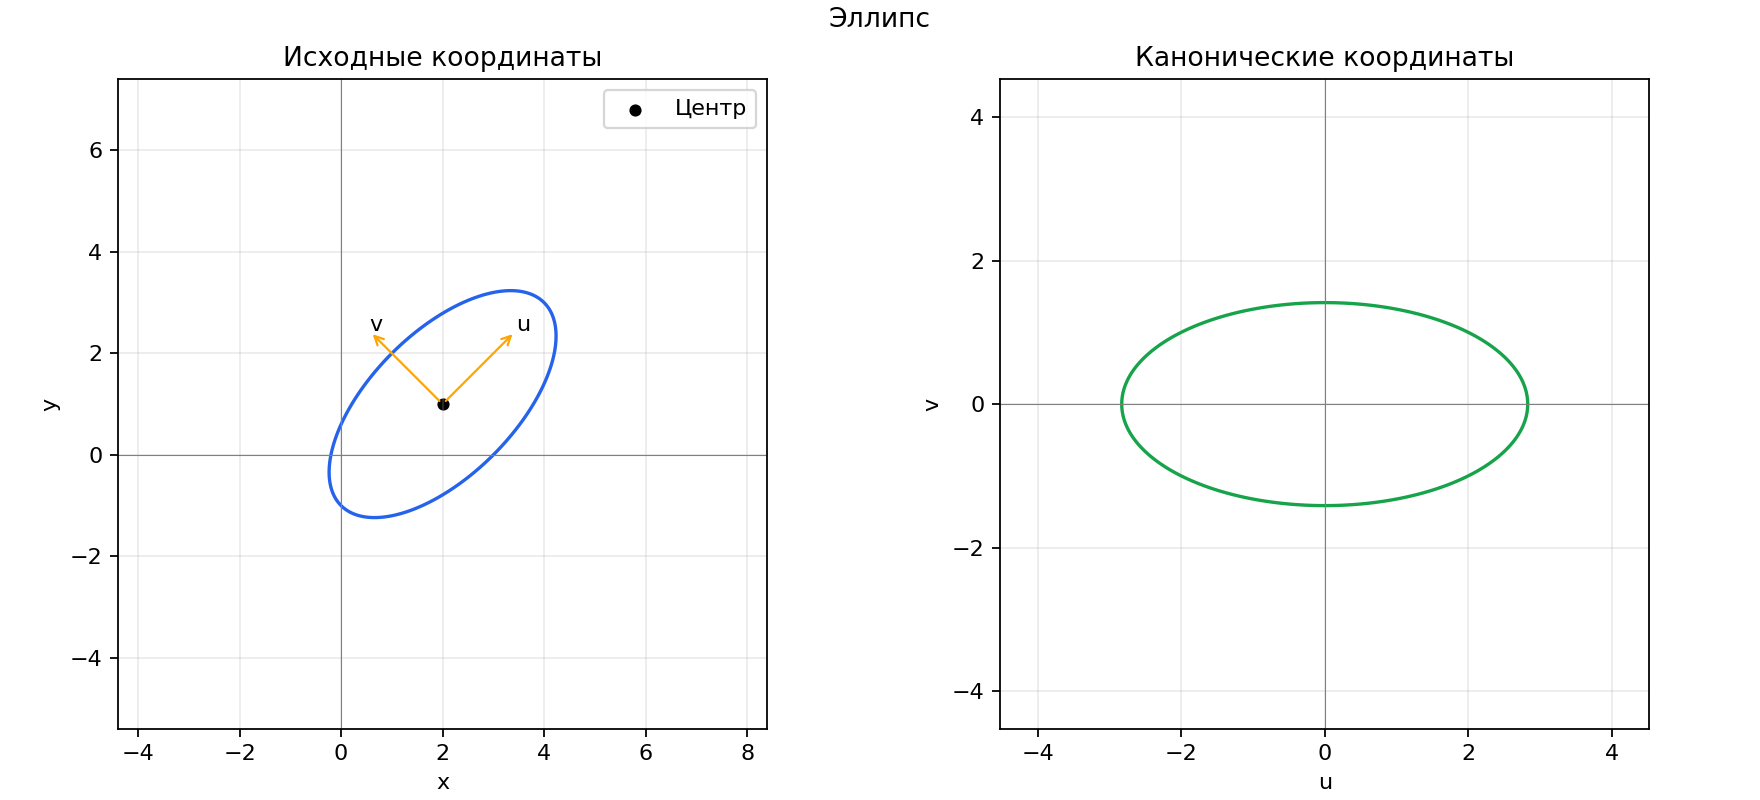
\includegraphics[width=0.94\textwidth]{examples/conic_01.png}
\end{center}
\textit{Пример: исходная кривая слева и каноническая справа.
Чёрная точка обозначает центр, стрелки --- направления новых осей.}


\newpage

\section{TF-IDF и поиск английских текстов}
\taskhead{Файлы для выполнения задач данного раздела}
\begin{itemize}
\item \func{solution.py} --- реализация текстовых функций, вычисления косинусной близости и ранжирования документов.
\item \func{data/documents.json} --- готовый корпус из 24 документов для итогового поискового эксперимента.
\item \func{demo_text.py} --- запуск поиска по готовому корпусу с использованием реализованных функций.
\item \func{run.py} и \func{tests/} --- запуск и материалы проверок \func{tokenize}, \func{tf}, \func{idf}, \func{tfidf}, \func{cosine} и \func{search} (группы 04--09).
\item \func{variant_check.py} --- данные своего варианта из приложений А.5--А.6, вызовы функций и дополнительные эксперименты. Изменённые копии корпуса для экспериментов следует создавать в этом скрипте, сохраняя исходный JSON-файл.
\item \func{report.tex} --- аналитические вычисления, таблицы сравнения и результаты поиска.
\end{itemize}

\begin{notabene}
  Корпус документов — совокупность текстовых документов, рассматриваемых совместно при обработке и анализе текста. В данной работе корпус используется для построения словаря, вычисления IDF и поиска документов, наиболее релевантных запросу.
\end{notabene}

\taskhead{Описание}
В данном разделе требуется реализовать восемь текстовых функций в \func{solution.py}.
Для этого использовать индивидуальный корпус из приложения А.5 для аналитических
вычислений и \func{data/documents.json} для итогового поискового эксперимента.
Основной корпус содержит 24 английских документа по два предложения: математика,
поиск текстов, программирование и повседневные ситуации. В индивидуальном варианте
используются четыре более коротких предложения. Каждый элемент JSON-массива
считается одним документом, независимо от количества предложений в нём.
Тесты запускаются из папки лабораторной работы.

{В предыдущих разделах координаты использовались для описания векторов и кривых. В задаче поиска текста аналогичный подход применим к текстам: 
документы и запрос представляются векторами, что позволяет сравнивать документы с помощью методов линейной алгебры.}

\taskhead{Порядок выполнения}
Задачи данного раздела 3.1--3.6 выполняются в следующем порядке:
\begin{enumerate}
\item Выделение слов и построение словаря.
\item Вычисление частот слов TF.
\item Вычисление обратных документных частот IDF.
\item Получение векторов TF-IDF.
\item Расчёт косинусной близости.
\item Ранжирование документов по близости к запросу.
\end{enumerate}
В задачах 3.1--3.4 и 3.6 использовать один корпус $d_1,d_2,d_3,d_4$
и запрос $q$ своего варианта из приложения А.5. Для задачи 3.5 использовать
пару векторов своего варианта из приложения А.6. Таким образом, каждая
задача данного раздела имеет 12 наборов исходных данных.

\taskhead{Теория}
Корпус --- конечная коллекция текстов. Словарь задаёт координаты:
каждое различное слово соответствует одной координате вектора.
TF характеризует частоту слова внутри документа, IDF --- его редкость
среди документов корпуса. Их произведение задаёт вес координаты.
Косинусная близость сравнивает направления векторов документов и запроса.
Такая модель не учитывает порядок слов: «dog bites man» и
«man bites dog» получают одинаковое представление.

\taskhead{Вводный пример NumPy}

Для ознакомления с основными операциями NumPy выполнить приведённый ниже код и проверить размерности полученных матриц. Рассмотренные операции потребуются при выполнении последующих заданий.

\begin{lstlisting}[style=commands]
import numpy as np
X = np.array([[1., 2., 3.], [4., 5., 6.]])
print(X.shape)         # (2, 3)
print(X[0])            # [1. 2. 3.]
print(X[:, 1])         # [2. 5.]
print(X.T.shape)       # (3, 2)
print(X * X)           # [[1,4,9], [16,25,36]]
print(X @ X.T)         # [[14,32], [32,77]]
print(X.sum(axis=0))   # [5,7,9]
print(X.sum(axis=1))   # [6,15]
sums = X.sum(axis=1, keepdims=True)
print(X / sums)        # each row divided by its sum
print(X + np.array([10., 20., 30.]))
\end{lstlisting}


\begin{itemize}
\item Оператор \func{*} выполняет поэлементное, а \func{@} --- матричное
умножение. 

\item Параметр \func{axis=0} суммирует по строкам, оставляя
результат для каждого столбца; \func{axis=1} --- по столбцам каждой строки.

\item Параметр \func{keepdims=True} сохраняет ось, по которой выполняется суммирование, с размером 1. 

\item При сложении
матрицы с вектором длины 3 NumPy прибавляет вектор к каждой строке. Следует выписать формы массивов перед вычислениями.

\end{itemize}

\newpage

\micro{Токенизация и словарь}
\taskhead{Теория}
Токен --- выделенная последовательность букв. 

\taskhead{Порядок выполнения}

\begin{enumerate}
  \item Взять четыре документа и запрос своего варианта
  из приложения А.5.
  \item Для каждого документа и запроса выписать список токенов:
  привести текст к нижнему регистру методом \func{casefold()},
  затем выделить все последовательности \func{[a-z]+}. 

  Пунктуацию, цифры и дефисы считать разделителями.
  Частые слова не удалять, словоформы не объединять.
  Например, текст «Cat, CAT-sleeps!» даёт список
  \func{['cat', 'cat', 'sleeps']}.
  \item Построить словарь уникальных токенов только
  по документам корпуса. Слова запроса при построении
  словаря не учитывать.
  Отсортировать слова по алфавиту и присвоить им
  индексы начиная с нуля.

  Например, для документов «cat cat sleeps» и «dog sleeps»
  словарь имеет вид \func|{"cat": 0, "dog": 1, "sleeps": 2}|.
  \item Реализовать функции \func{tokenize}
  и \func{build_vocabulary}.
  \item Проверить реализацию, выполнив команду:
  \begin{lstlisting}[style=commands]
  python run.py unittest tokenize\end{lstlisting}
  \item Вызвать функции на данных своего варианта.
  Сопоставить полученные списки токенов и словарь
  с результатами самостоятельного разбора.
  Проверить точное совпадение слов, их порядка
  и присвоенных индексов.
\end{enumerate}

\underline{Ожидаемый результат}: точное совпадение списков токенов и словаря
с аналитическим ответом. Для пустого списка документов в \func{build_vocabulary}
должно быть возбуждено исключение \func{ValueError}; непустой корпус без слов может иметь пустой словарь.

{
\taskhead{Пример}

В предыдущих разделах основное внимание уделялось
аналитическим вычислениям и их программной реализации.
Ниже приведён пример использования ИИ для подготовки
отдельного блока кода на основе сформулированного
задания.

При составлении запроса к ИИ последовательно указываются исходные
данные, требуемые действия, ограничения и формат результата.
Формулировки должны однозначно определять правила обработки
текста и построения словаря. При решении данной задаче в промпте указывается,
что словарь строится только по документам корпуса, без учёта
поискового запроса, а индексы присваиваются словам
в алфавитном порядке.

Использование ИИ не заменяет самостоятельного разбора задачи:
полученный код необходимо проверить на работоспособность, объяснить принцип его
работы и сопоставить результаты с предварительно
выполненными вычислениями.

\newpage

Пример промпта к ИИ для генерации кода:

% Промпт является обычным текстом: переносы выполняются по словам.
\par\begingroup
\setlength{\fboxsep}{10pt}
\noindent\colorbox{gray!10}{%
\begin{minipage}{\dimexpr\linewidth-2\fboxsep\relax}
\small\ttfamily\raggedright
\setlength{\parskip}{6pt}
Для набора документов и запроса напиши мне блок кода на python, выполняющий следующие задачи:

Для каждого документа и запроса выпиши список токенов, заранее приведя текст в нижний регистр с помощью функций python и примени регулярное выражение "[a-z]+". Пробелы, пунктуацию, цифры и дефисы считать разделителями. Текст в каждом документе преобразуй в список слов. На основе данного списка построй словарь уникальных токенов, отсортируй токены по алфовиту и присвой каждому индексы, начиная с нуля.

Мои исходные данные:

d1: The young fox rests near the tree.\\
d2: The young deer rests near the river.\\
d3: The fox watches the young deer.\\
d4: The deer watches birds near the tree.\\
q: young fox tree
\end{minipage}%
}
\par\endgroup

Ответ ИИ:

\begin{lstlisting}[style=commands,escapeinside={(*@}{@*)}]
import re

documents = [
    "The young fox rests near the tree.",
    "The young deer rests near the river.",
    "The fox watches the young deer.",
    "The deer watches birds near the tree.",
]
query = "young fox tree"


def tokenize(text):
    return re.findall(r"[a-z]+", text.casefold())


document_tokens = [tokenize(document) for document in documents]
query_tokens = tokenize(query)

unique_tokens = sorted({
    token
    for tokens in document_tokens
    for token in tokens
}) # Словарь строится только по документам, без добавления запроса.
vocabulary = {
    token: index
    for index, token in enumerate(unique_tokens)
}

for index, tokens in enumerate(document_tokens, start=1):
    print(f"d{index}: {tokens}")

print(f"q: {query_tokens}")
(*@\texttt{\detokenize{print(f"Словарь: {vocabulary}")}}@*)
\end{lstlisting}

В приведённом примере результатом обращения к ИИ является
самостоятельный блок кода, соответствующий запрошенному формату.
Для включения в лабораторную работу проверить его корректность
и перенести нужные операции в функции \func{tokenize}
и \func{build_vocabulary} файла \func{solution.py}.
Сохранить заданные имена функций, аргументы и форматы
возвращаемых результатов. Документы конкретного варианта
передавать через аргументы, а не задавать внутри функций.
После адаптации выполнить требования, приведенные в "Порядке выполнения".}

\micro{Частоты слов TF}
\taskhead{Теория}


TF (Term Frequency) --- частота термина в документе.
В данной работе она определяется как отношение числа
вхождений токена к общему количеству токенов документа:
\[
\operatorname{TF}(t,d)=\frac{c(t,d)}{L_d},
\]

где $c(t,d)$ --- число вхождений токена $t$ в документе $d$, $L_d$ --- количество токенов в документе $d$.

\taskhead{Задача данного раздела, порядок выполнения и проверка}

\begin{enumerate}
  \item Подсчитать токены в каждом документе и запросе своего варианта из приложения А.5.
  \item Составить таблицу абсолютных частот. Каждый элемент строки разделить
  на общее количество токенов соответствующего документа или запроса с учётом повторений.
  \item Реализовать \func{term_frequency(tokens, vocabulary)}.
  Для пустого текста функция возвращает нулевой вектор.
  \item Проверить реализацию, выполнив команду:
  \begin{lstlisting}[style=commands]
  python run.py unittest tf\end{lstlisting}
  \item Вызвать функцию на данных своего варианта.
  Сопоставить точные значения в виде дробей и программные значения
  в одном порядке координат; вычислить абсолютную и относительную ошибки.
\end{enumerate}

\underline{Ожидаемый результат}: четыре вектора документов и вектор запроса размера $V$,
где $V$ --- размер словаря. Привести точные значения в виде дробей и программные значения
в одном порядке координат. Вычислить абсолютную и относительную ошибки.

\taskhead{Пример}

В словаре $(\text{cat},\text{dog},\text{sleeps})$ текст «cat cat sleeps»
имеет TF $(2/3,0,1/3)$, а «dog sleeps» --- $(0,1/2,1/2)$.
Неизвестные слова не создают координат, но входят в знаменатель:
«cat unknown» имеет TF $(1/2,0,0)$.

\micro{Обратные документные частоты IDF}
\taskhead{Теория}

IDF (Inverse Document Frequency) --- обратная частота
документа. Она характеризует редкость термина в корпусе:
чем меньше документов содержат термин, тем выше его IDF.

Пусть $N$ --- число документов, а $\operatorname{df}(t)$ ---
число документов, содержащих слово $t$ хотя бы один раз.
Каждый такой документ увеличивает $\operatorname{df}(t)$
на единицу независимо от числа вхождений слова в него. Для подсчета $IDF$ используется формула:

\[
\operatorname{IDF}(t)=\ln\frac{N+1}{\operatorname{df}(t)+1}+1,
\]

где $\operatorname{ln}$ --- натуральный логарифм. В NumPy использовать \func{np.log}.


Добавление единицы в числитель и знаменатель обеспечивает сглаживание
и исключает деление на ноль. Дополнительное слагаемое 1 обеспечивает
значение IDF, равное единице, для слова, присутствующего во всех документах.

\taskhead{Порядок выполнения}
\begin{enumerate}
  \item Взять четыре документа своего варианта из приложения А.5
  и словарь, построенный в пункте 3.1.
  Запрос в корпус не включать.
  \item Для каждого слова словаря определить аналитически
  документную частоту $\operatorname{df}(t)$.
  Составить таблицу присутствия слов в документах:
  указать 1, если слово встречается в документе, и 0 иначе.
  Суммировать значения по документам для каждого слова.
  \item Вычислить IDF каждого слова по формуле
  \[
  \operatorname{IDF}(t)
  =\ln\frac{N+1}{\operatorname{df}(t)+1}+1
  \]
  Привести точные выражения с логарифмами и приближённые
  значения не менее чем с шестью знаками после запятой.
  \item Реализовать функцию \func{inverse_document_frequency}.
  При подсчёте документной частоты учитывать каждое слово
  не более одного раза в каждом документе.
  Расположить значения IDF в порядке индексов словаря.
  \item Проверить реализацию, выполнив команду:
  \begin{lstlisting}[style=commands]
python run.py unittest idf\end{lstlisting}
  \item Вызвать функцию на документах своего варианта.
  Сопоставить аналитический и программный векторы IDF,
  вычислить абсолютную и относительную ошибки.
  Для сравнения использовать значения до округления.
\end{enumerate}

\underline{Ожидаемый результат}: таблица присутствия слов,
вектор документных частот, аналитический и программный
векторы IDF, абсолютная и относительная ошибки,
а также успешное прохождение тестов.

\newpage

\taskhead{Пример}

Для корпуса из двух документов «cat cat sleeps» и «dog sleeps»
при порядке слов $(\text{cat},\text{dog},\text{sleeps})$
вектор документных частот равен $(1,1,2)$:
«cat» и «dog» встречаются в одном документе каждый,
а «sleeps» --- в обоих.

При $N=2$ вектор IDF имеет вид
\[
\left(1+\ln\frac{3}{2},\;1+\ln\frac{3}{2},\;1\right).
\]

Подсчёт для того же примера можно оформить таблицей:
\begin{center}
\begin{tabular}{lccccc}
Слово & $c(t,d_1)$ & $c(t,d_2)$ & $\operatorname{df}(t)$ & $\operatorname{TF}(t,d_1)$ & IDF\\\hline
cat & 2 & 0 & 1 & $2/3$ & $1+\ln(3/2)$\\
dog & 0 & 1 & 1 & $0$ & $1+\ln(3/2)$\\
sleeps & 1 & 1 & 2 & $1/3$ & $1$\\
\end{tabular}
\end{center}
Длина $d_1$ равна 3, длина $d_2$ --- 2. Слово cat встретилось дважды,
но только в одном документе, поэтому его df равно 1, а не 2.
Для sleeps получаем $\ln((2+1)/(2+1))+1=\ln1+1=1$.
Этот демонстрационный корпус содержит два документа, а индивидуальные
варианты --- четыре. В варианте при расчёте IDF подставить $N=4$.

\micro{Векторизация TF-IDF}

\taskhead{Теория}

Векторизация TF-IDF --- представление документа числовым
вектором, координаты которого соответствуют словам словаря.


Вес каждого слова вычисляется как
\[
x_{dj}=\operatorname{TF}(t_j,d)\operatorname{IDF}(t_j).
\]
Если слово отсутствует в документе, его вес равен нулю.

Векторы документов образуют строки матрицы
$X\in\mathbb{R}^{N\times V}$, где $N$ --- число документов,
а $V$ --- размер словаря. Порядок слов одинаков для всех строк.
Каждый столбец матрицы TF умножается на соответствующее
значение IDF; в NumPy это операция \func{tf_matrix * idf}.

\newpage

\taskhead{Порядок выполнения}
\begin{enumerate}
  \item Взять четыре документа и запрос своего варианта
  из приложения А.5. Использовать словарь, значения TF
  и IDF, полученные в пунктах 3.1--3.3.
  \item Вычислить аналитически TF-IDF-векторы документов
  и запроса: умножить каждую частоту TF
  на соответствующее значение IDF.
  Записать векторы документов строками матрицы
  в порядке следования документов.
  \item Реализовать \func{tfidf_fit}:
  построить словарь и вычислить IDF по корпусу,
  сформировать матрицу TF-IDF.
  Вернуть \func{(vocabulary, idf, matrix)}.
  Использовать ранее реализованные функции.
  \item Реализовать \func{tfidf_transform}:
  преобразовать новые тексты с использованием
  готового словаря и вектора IDF.
  Словарь не изменять, IDF не пересчитывать.
  Дополнительную нормировку векторов не выполнять.
  \item Проверить реализацию, выполнив команду:
  \begin{lstlisting}[style=commands]
python run.py unittest tfidf\end{lstlisting}
  \item Вызвать \func{tfidf_fit} на документах своего варианта,
  затем преобразовать запрос с помощью
  \func{tfidf_transform}, передав его списком из одной строки.
  Проверить размеры результатов: $(4,V)$ для документов
  и $(1,V)$ для запроса, где $V$ --- размер словаря.
  \item Сопоставить аналитические и программные результаты.
  Вычислить абсолютную и относительную ошибки отдельно
  для матрицы документов и вектора запроса.
\end{enumerate}

\underline{Ожидаемый результат}: матрица TF-IDF четырёх
документов размера $(4,V)$ и представление запроса
размера $(1,V)$ в общем словаре, где $V$ --- размер словаря.
Для обоих результатов приводятся аналитические
и программные значения, абсолютная и относительная
ошибки. Все тесты должны быть пройдены.

\begin{notabene}
При передаче пустого списка новых текстов функция
\func{tfidf_transform} должна возвращать массив
формы $(0,V)$. Исходные словарь и IDF не изменяются.
\end{notabene}

\taskhead{Пример}

Рассмотрим документы $d_1$: «cat cat sleeps»
и $d_2$: «dog sleeps». При порядке слов
$(\text{cat},\text{dog},\text{sleeps})$ их векторы TF равны
\[
\operatorname{TF}_1=(2/3,0,1/3),\qquad
\operatorname{TF}_2=(0,1/2,1/2).
\]
Вектор IDF этого корпуса равен $(w,w,1)$,
где $w=1+\ln(3/2)\approx1.405465$.

Умножим каждую координату TF на соответствующее значение IDF:
\[
x_1=(\tfrac23w,0,\tfrac13),\qquad
x_2=(0,\tfrac12w,\tfrac12).
\]
Записав векторы документов строками, получим матрицу TF-IDF:
\[
X=
\begin{pmatrix}
\frac23w & 0 & \frac13\\
0 & \frac12w & \frac12
\end{pmatrix}
\approx
\begin{pmatrix}
0.936977 & 0 & 0.333333\\
0 & 0.702733 & 0.5
\end{pmatrix}.
\]

Для запроса «cat» вектор TF равен $(1,0,0)$.
Используя тот же вектор IDF, получим
\[
q=(w,0,0)\approx(1.405465,0,0).
\]
Словарь и IDF при обработке запроса не изменяются.
Дополнительная нормировка векторов не выполняется.


\micro{Косинусная близость}

\taskhead{Теория}

Косинусная близость --- мера сходства направлений двух
ненулевых векторов одной размерности. Она равна косинусу
угла между ними:
\[
\operatorname{cos}(a,b)=\frac{a^Tb}{\|a\|\|b\|},
\]
где $a^Tb$ --- скалярное произведение, а $\|a\|$ и $\|b\|$
--- евклидовы нормы векторов:
\[
a^Tb=\sum_j a_jb_j,\qquad
\|a\|=\sqrt{\sum_j a_j^2},\qquad
\|b\|=\sqrt{\sum_j b_j^2}.
\]

Косинусная близость принимает значения от $-1$ до $1$:
\begin{itemize}
  \item $1$ --- векторы сонаправлены;
  \item $0$ --- векторы перпендикулярны;
  \item $-1$ --- векторы противоположно направлены.
\end{itemize}
Умножение любого из векторов на положительное число
не изменяет косинусную близость: она зависит
от направлений векторов, а не от их длин.

Для TF-IDF-векторов все координаты неотрицательны,
поэтому близость лежит в диапазоне $[0,1]$.
Чем выше близость вектора документа к вектору запроса,
тем выше оценивается релевантность документа в данной модели.
Значение $1$ означает совпадение направлений векторов,
но не обязательно совпадение исходных текстов.

Если хотя бы один вектор нулевой, угол и косинус
математически не определены. В данной работе для такого
случая принимается соглашение возвращать близость $0$.

\begin{notabene}{
  \setlength{\parskip}{8pt}Косинусная близость двух ненулевых векторов не изменяется
  при их повороте на один и тот же угол вокруг одной оси,
  проходящей через начало координат. Такой поворот сохраняет
  длины векторов и угол между ними.

  Умножение одной и той же координаты обоих векторов
  на одинаковый положительный коэффициент
  изменяет косинусную близость в общем случае. В отличие от равномерного
  масштабирования всех координат, такое преобразование
  может изменить угол между векторами.

  Например, для $a=(1,1)$ и $b=(1,0)$ близость равна
  $1/\sqrt{2}$. После удвоения первой координаты
  получаются векторы $a'=(2,1)$ и $b'=(2,0)$, для которых
  \[
  \operatorname{cos}(a',b')
  =\frac{4}{2\sqrt{5}}
  =\frac{2}{\sqrt{5}}
  \ne\frac{1}{\sqrt{2}}.
  \]
  Следовательно, изменение весов отдельных координат,
  в том числе при умножении TF на IDF, может изменить
  косинусную близость документов и запроса.
}\end{notabene}

\taskhead{Порядок выполнения}
\begin{enumerate}
  \item Взять векторы $a$ и $b$ своего варианта
  из приложения А.6.
  \item Вычислить аналитически скалярное произведение
  $a^Tb$, нормы $\|a\|$ и $\|b\|$, затем косинусную близость.
  Привести промежуточные вычисления, точное значение
  и его приближение не менее чем с шестью знаками
  после запятой.
  \item Реализовать \func{cosine_similarity(a, b)}
  для векторов одной размерности.
  Если хотя бы один вектор нулевой, возвращать $0$.
  \item Проверить реализацию, выполнив команду:
  \begin{lstlisting}[style=commands]
python run.py unittest cosine\end{lstlisting}
  \item Вызвать функцию на векторах своего варианта.
  Сопоставить аналитический и программный результаты,
  вычислить абсолютную и относительную ошибки.
  При нулевом аналитическом результате указать
  только абсолютную ошибку.
  \item Сравнить косинусную близость пар $(a,b)$ и $(2a,b)$
  аналитически и программно. Объяснить равенство результатов.
  \item Проверить, что для пары $(0,b)$ функция возвращает $0$,
  где $0$ --- нулевой вектор той же размерности, что и $b$.
\end{enumerate}

\underline{Ожидаемый результат}: аналитическое
и программное значения косинусной близости,
абсолютная и относительная ошибки, корректная обработка
нулевого вектора и успешное прохождение тестов.

\taskhead{Пример}

Рассмотрим векторы $a=(1,1)$ и $b=(1,0)$.
Вычислим скалярное произведение:
\[
a^Tb=1\cdot1+1\cdot0=1.
\]
Нормы векторов равны
\[
\|a\|=\sqrt{1^2+1^2}=\sqrt2,\qquad
\|b\|=\sqrt{1^2+0^2}=1.
\]
Следовательно, косинусная близость составляет
\[
\operatorname{cos}(a,b)
=\frac{1}{\sqrt2\cdot1}
=\frac{1}{\sqrt2}\approx0.707107.
\]
Это соответствует углу $45^\circ$ между векторами.

Умножим первый вектор на 2: $2a=(2,2)$.
Тогда
\[
\operatorname{cos}(2a,b)
=\frac{2\cdot1+2\cdot0}{\sqrt{2^2+2^2}\cdot1}
=\frac{2}{2\sqrt2}
=\frac{1}{\sqrt2}.
\]
Длина вектора изменилась, но его направление
и косинусная близость остались прежними.

Для пары $(0,0)$ и $b=(1,0)$ формула содержит деление
на ноль. В соответствии с принятым в работе соглашением
функция должна вернуть $0$.

\micro{Поиск и ранжирование документов}
\taskhead{Теория}

Ранжирование документов --- упорядочивание документов
по степени их соответствия поисковому запросу.
В данной работе соответствие оценивается косинусной
близостью TF-IDF-векторов документа и запроса:
\[
s_i=\operatorname{cos}(x_i,q),
\]
где $x_i$ --- вектор документа, а $q$ --- вектор запроса.

Запрос преобразуется с использованием словаря
и значений IDF корпуса. Документы упорядочиваются
по убыванию оценки $s_i$.
При равенстве оценок первым располагается документ
с меньшим индексом. Программные индексы начинаются с нуля.

Параметр \func{top_k} задаёт максимальное число
возвращаемых документов. Результат поиска представляет
собой упорядоченный список из \func{min(top_k, N)} пар
\func{(index, score)}, где $N$ --- число документов.
Документы с нулевыми оценками также включаются
в результат в пределах указанного количества.

Если запрос не содержит слов из словаря,
его вектор нулевой. По принятому соглашению
все оценки равны нулю, а документы упорядочиваются
по возрастанию индексов.

Данная модель учитывает совпадение слов и их веса,
но не учитывает порядок слов и смысловые связи между ними.
Поэтому высокая оценка характеризует сходство
векторных представлений, но не гарантирует соответствие
содержания документа смыслу запроса.

\taskhead{Порядок выполнения}
\begin{enumerate}
  \item Взять четыре документа и запрос своего варианта
  из приложения А.5. Использовать их TF-IDF-представления,
  полученные в пункте 3.4.
  \item Вычислить аналитически косинусную близость
  запроса с каждым документом. Привести промежуточные
  вычисления и четыре итоговые оценки.
  Упорядочить документы по убыванию оценок,
  а при равенстве --- по возрастанию индексов.
  \item Реализовать \func{rank_documents},
  используя ранее реализованные функции.
  Результат представить списком пар \func{(index, score)}.

  Возвращать \func{min(top_k, N)} пар, включая пары
  с нулевыми оценками. При \func{top_k=0}
  возвращать пустой список.
  \item Проверить реализацию и весь текстовый раздел,
  выполнив команды:
  \begin{lstlisting}[style=commands]
python run.py unittest search
python run.py --part text\end{lstlisting}
  \item Вызвать функцию на данных своего варианта
  с параметром \func{top_k=4}.
  Сопоставить аналитические и программные оценки,
  вычислить абсолютную и относительную ошибки
  для вектора четырёх оценок.
  При сравнении расположить оценки в исходном порядке
  документов. Отдельно проверить совпадение
  порядка документов после ранжирования.
  \item Повторить каждое слово запроса дважды
  и сравнить результаты поиска с исходными.
  Объяснить, почему оценки и порядок документов
  должны сохраниться.
  \item Выполнить запрос «zzzzunknown».
  Проверить нулевые оценки всех документов
  и их расположение по возрастанию индексов.
  \item Добавить в корпус копию первого документа.
  Повторно вычислить IDF и TF-IDF-представления,
  выполнить поиск по исходному запросу.
  Объяснить изменения весов и результатов поиска.
  \item Выполнить поиск по готовому корпусу
  \func{data/documents.json}:
  \begin{lstlisting}[style=commands]
python demo_text.py "matrix vector"
python demo_text.py "neural network"
python demo_text.py "cat"\end{lstlisting}
  Для каждого запроса сохранить первые три результата:
  индексы документов, их тексты и оценки.
  Кратко объяснить соответствие найденных документов запросу.
\end{enumerate}

\underline{Ожидаемый результат}: четыре аналитические
и программные оценки для своего варианта,
абсолютная и относительная ошибки,
совпадение порядка документов после ранжирования,
результаты дополнительных проверок и поиска
по готовому корпусу, а также успешное прохождение тестов.

\taskhead{Пример}

Рассмотрим документы $d_1$: «cat cat sleeps»,
$d_2$: «dog sleeps» и запрос «cat».
При порядке слов $(\text{cat},\text{dog},\text{sleeps})$
их TF-IDF-векторы равны
\[
x_1=(\tfrac23w,0,\tfrac13),\qquad
x_2=(0,\tfrac12w,\tfrac12),\qquad
q=(w,0,0),
\]
где $w=1+\ln(3/2)$.

Вычислим оценку соответствия первого документа запросу:
\[
s_1=\frac{x_1^Tq}{\|x_1\|\|q\|}
=\frac{\frac23w^2}
{\sqrt{\frac49w^2+\frac19}\cdot w}
=\frac{2w}{\sqrt{4w^2+1}}
\approx0.942156.
\]
Для второго документа скалярное произведение равно нулю:
\[
x_2^Tq=0,\qquad s_2=0.
\]
Следовательно, порядок документов по убыванию оценки:
$d_1$, затем $d_2$. При \func{top_k=2} функция возвращает
список пар с программными индексами:
\[
[(0,\;0.942156),\;(1,\;0)].
\]
Оценка первого документа приведена с округлением.
При \func{top_k=1} возвращается только первая пара.

Для запроса «zzzzunknown» вектор $q$ равен нулю,
поскольку слово отсутствует в словаре.
Оба документа получают оценку $0$ и располагаются
по возрастанию индексов:
\[
[(0,\;0),\;(1,\;0)].
\]

\newpage

\section{Требования к отчёту и составу сдаваемых материалов}

Отчет предоставляется к защите в формате LaTeX в виде исходного tex-файла и PDF-файла. 
В отчете должны быть приведены все аналитические вычисления, результаты вызова функций и их сравнение с аналитическими расчетами. Рисунки должны иметь подписи и ссылки в тексте.

Краткий контрольный список для подготовки отчёта приведён в файле \func{report_template.tex}.

\taskhead{Структура отчета}

\begin{enumerate}
\item \textbf{Титульный лист.} Указать название работы, тему, ФИО участников команды, номер группу
и номер варианта.
\item \textbf{Цель и технические характеристики.} Сформулировать цель своими словами.
Дополнительно указать ОС, версии Python и NumPy.
\item \textbf{Порядок выполнения.} Привести краткую последовательность выполненных шагов разделов 1--3.
\item \textbf{Раздел 1.} Оформить все задачи раздела 1: вычисление определителя, решение СЛАУ методом Крамера и определение координат вектора в новом базисе. 
Для каждой задачи привести исходные данные, подробные аналитические вычисления,
вызов своей функции, её результат, сравнение и вывод.
Для метода Крамера указать все заменённые определители; для координат выписать разложение по базисным векторам. Для каждой задачи указать
абсолютную и относительную ошибки; для СЛАУ и смены базиса ---
векторы невязок и максимальные модули их компонент.
\item \textbf{Раздел 2.} Привести исходное уравнение, обоснование поворота
или его отсутствия, подстановку, выделение квадратов, перенос,
каноническое уравнение, обе замены координат и характеристики кривой.
Решение сопровождается проверкой двух контрольных точек с полными подстановками и двумя рисунками.
\item \textbf{Раздел 3.} Оформить шесть подразделов по задачам данного раздела.
Привести токены и словарь; таблицы счётчиков и TF; df и IDF;
матрицу TF-IDF и вектор запроса; отдельный расчёт косинуса из приложения А.6;
четыре поисковые оценки и порядок документов после ранжирования. Для каждого этапа сопоставить
аналитические и программные ответы. Раздел завершается результатами экспериментов.
\item \textbf{Проверка реализации.} Представить результаты тестирования
в таблице со столбцами: "название задачи", "команда запуска",
"статус выполнения" и "\underline{количество пройденных тестов}".
Включить в отчет результаты проверок, предусмотренных условием.
Полный журнал выполнения тестов в отчёт не включать.
\item \textbf{Заключение.} Привести описание полученных результатов, обнаруженных
расхождений и способов их устранения. Требуется объяснить ограничения косинусного
поиска и роль проверки подстановкой. При использовании внешних материалов (заимствованные части кода, взятые с интернет-ресурсов; ссылки на документацию NumPy в случае использования функций, не описанных в условиях лабораторной работы)
привести список источников.
\end{enumerate}

\newpage

\taskhead{Формат сравнения результатов}

\begin{itemize}
\item Для оформления численных результатов разделов 1 и 3 использовать таблицу следующего вида:
\begin{center}
\begin{tabular}{|l|l|l|l|l|}\hline
Величина & Аналитически & Программа & Абс. ошибка & Отн. ошибка\\\hline
$\det A$ & $-6$ & $-6.000000$ & $0$ & $0$\\\hline
\end{tabular}
\end{center}

\item Для массивов сравнить элементы в одинаковом порядке и указать
ошибки $\Delta$ и $\delta$ по формулам, приведённым в конце настоящего раздела.
Если относительная ошибка не определена, в таблице ставится прочерк.
Для СЛАУ и смены базиса отдельно приводятся вектор невязки и максимальный модуль его компонент.
Для токенов, словаря и порядка документов указать точное совпадение
или конкретное различие. 

\item Нельзя ограничиваться фразой «всё совпало» --- в выводе необходимо представить, как минимум, результаты вычислений и их качественное сравнение. 

\item Указать формулы и подстановки, по которым
получен аналитический результат; программный вывод сам по себе аналитическими вычислениями не является.

\item Рисунки раздела 2 должны иметь подписи и ссылки в тексте. На рисунках обозначить
координатные оси, центр или вершину кривой, направления новых осей и характерные
точки. Выбрать масштаб, позволяющий проверить геометрию кривой;
сохранить равные единицы длины по обеим осям.

\item Файл \func{variant_check.py} создать рядом с \func{solution.py}.
В \func{variant_check.py} разместить вызовы функций своего варианта
и вывод сравниваемых величин. Импортировать вычисления из
\func{solution.py}; не дублировать алгоритмы в проверочном скрипте.
Названия рисунков могут отличаться; использовать относительные пути
в \func{report.tex}. Допускаются PDF-рисунки.

\item Не включать окружение, кеши и служебные файлы сборки. Проверить сборку PDF из передаваемых исходников.

\end{itemize}


\taskhead{Комплект для сдачи лабораторной работы}
\begin{verbatim}
submission/
  solution.py
  variant_check.py
  report.tex
  report.pdf
  figures/
    original_curve.png
    canonical_curve.png
\end{verbatim}

\newpage

\taskhead{Абсолютная и относительная ошибки. Невязка}
\begin{itemize}
\item Для сравнения аналитического результата $z$ и программного результата
$\widehat z$ указать абсолютную и относительную ошибки:
\[
\Delta=|\widehat z-z|,\qquad \delta=\frac{\Delta}{|z|}.
\]
Для векторов использовать формулы
\[
\Delta=\max_i|\widehat z_i-z_i|,\qquad
\delta=\frac{\Delta}{\max_i|z_i|}.
\]
Для матриц брать максимальное значение по всем элементам. Если аналитический результат
равен нулю (для массива --- все элементы равны нулю), относительная ошибка
не определяется; указывается только абсолютная ошибка.

Использовать неокруглённые значения при вычислениях;
для малых примеров этой работы ориентироваться на абсолютную ошибку
не более $10^{-8}$. При сравнении округлённых значений точность округления указывать явно.
\item Невязка характеризует выполнение исходных уравнений и не совпадает
с ошибкой относительно аналитического решения. Для СЛАУ невязка равна
\[
r=A\widehat x-b.
\]
Для смены базиса:
\[
r=P\widehat c-x,
\]
где $\widehat x$ и $\widehat c$ получены программно.
В этих задачах в отчете привести вектор невязки и максимальный модуль его компонент
$\max_i|r_i|$.
\end{itemize}

\clearpage
\section*{Приложение А. Индивидуальные варианты}



\par\ifdim\dimexpr\pagegoal-\pagetotal\relax<140pt\relax\newpage\fi
\subsection*{А.1. Определитель: для задач раздела 1.1}
{\small
\begin{longtable}{@{}p{0.30\textwidth}p{0.30\textwidth}p{0.30\textwidth}@{}}
\begin{minipage}[t]{\linewidth}\vspace{0pt}\raggedright\setlength{\parskip}{0pt}
\textbf{Вариант 1.}\par\smallskip
\(\displaystyle A_k=\begin{pmatrix}0&1&1\\1&2&0\\2&1&2\end{pmatrix}\)\par
\end{minipage} &
\begin{minipage}[t]{\linewidth}\vspace{0pt}\raggedright\setlength{\parskip}{0pt}
\textbf{Вариант 2.}\par\smallskip
\(\displaystyle A_k=\begin{pmatrix}0&2&1\\1&2&0\\2&1&3\end{pmatrix}\)\par
\end{minipage} &
\begin{minipage}[t]{\linewidth}\vspace{0pt}\raggedright\setlength{\parskip}{0pt}
\textbf{Вариант 3.}\par\smallskip
\(\displaystyle A_k=\begin{pmatrix}0&3&1\\1&2&0\\2&1&4\end{pmatrix}\)\par
\end{minipage}\\\noalign{\vskip 14pt}
\begin{minipage}[t]{\linewidth}\vspace{0pt}\raggedright\setlength{\parskip}{0pt}
\textbf{Вариант 4.}\par\smallskip
\(\displaystyle A_k=\begin{pmatrix}0&4&1\\1&2&0\\2&1&5\end{pmatrix}\)\par
\end{minipage} &
\begin{minipage}[t]{\linewidth}\vspace{0pt}\raggedright\setlength{\parskip}{0pt}
\textbf{Вариант 5.}\par\smallskip
\(\displaystyle A_k=\begin{pmatrix}0&5&1\\1&2&0\\2&1&6\end{pmatrix}\)\par
\end{minipage} &
\begin{minipage}[t]{\linewidth}\vspace{0pt}\raggedright\setlength{\parskip}{0pt}
\textbf{Вариант 6.}\par\smallskip
\(\displaystyle A_k=\begin{pmatrix}0&6&1\\1&2&0\\2&1&7\end{pmatrix}\)\par
\end{minipage}\\\noalign{\vskip 14pt}
\begin{minipage}[t]{\linewidth}\vspace{0pt}\raggedright\setlength{\parskip}{0pt}
\textbf{Вариант 7.}\par\smallskip
\(\displaystyle A_k=\begin{pmatrix}0&7&1\\1&2&0\\2&1&8\end{pmatrix}\)\par
\end{minipage} &
\begin{minipage}[t]{\linewidth}\vspace{0pt}\raggedright\setlength{\parskip}{0pt}
\textbf{Вариант 8.}\par\smallskip
\(\displaystyle A_k=\begin{pmatrix}0&8&1\\1&2&0\\2&1&9\end{pmatrix}\)\par
\end{minipage} &
\begin{minipage}[t]{\linewidth}\vspace{0pt}\raggedright\setlength{\parskip}{0pt}
\textbf{Вариант 9.}\par\smallskip
\(\displaystyle A_k=\begin{pmatrix}0&9&1\\1&2&0\\2&1&10\end{pmatrix}\)\par
\end{minipage}\\\noalign{\vskip 14pt}
\begin{minipage}[t]{\linewidth}\vspace{0pt}\raggedright\setlength{\parskip}{0pt}
\textbf{Вариант 10.}\par\smallskip
\(\displaystyle A_k=\begin{pmatrix}0&10&1\\1&2&0\\2&1&11\end{pmatrix}\)\par
\end{minipage} &
\begin{minipage}[t]{\linewidth}\vspace{0pt}\raggedright\setlength{\parskip}{0pt}
\textbf{Вариант 11.}\par\smallskip
\(\displaystyle A_k=\begin{pmatrix}0&11&1\\1&2&0\\2&1&12\end{pmatrix}\)\par
\end{minipage} &
\begin{minipage}[t]{\linewidth}\vspace{0pt}\raggedright\setlength{\parskip}{0pt}
\textbf{Вариант 12.}\par\smallskip
\(\displaystyle A_k=\begin{pmatrix}0&12&1\\1&2&0\\2&1&13\end{pmatrix}\)\par
\end{minipage}\\\noalign{\vskip 14pt}
\end{longtable}
}

\par\ifdim\dimexpr\pagegoal-\pagetotal\relax<140pt\relax\newpage\fi
\subsection*{А.2. Метод Крамера: для задач раздела 1.2}
{\small
\begin{longtable}{@{}p{0.46\textwidth}p{0.46\textwidth}@{}}
\begin{minipage}[t]{\linewidth}\vspace{0pt}\raggedright\setlength{\parskip}{0pt}
\textbf{Вариант 1.}\par\smallskip
\(\displaystyle B_k=\begin{pmatrix}3&1&0\\1&4&1\\0&1&5\end{pmatrix},\quad b_k=\begin{pmatrix}1\\3\\-4\end{pmatrix}\)\par
\end{minipage} &
\begin{minipage}[t]{\linewidth}\vspace{0pt}\raggedright\setlength{\parskip}{0pt}
\textbf{Вариант 2.}\par\smallskip
\(\displaystyle B_k=\begin{pmatrix}4&1&0\\1&5&1\\0&1&6\end{pmatrix},\quad b_k=\begin{pmatrix}6\\11\\2\end{pmatrix}\)\par
\end{minipage}\\\noalign{\vskip 14pt}
\begin{minipage}[t]{\linewidth}\vspace{0pt}\raggedright\setlength{\parskip}{0pt}
\textbf{Вариант 3.}\par\smallskip
\(\displaystyle B_k=\begin{pmatrix}5&1&0\\1&6&1\\0&1&7\end{pmatrix},\quad b_k=\begin{pmatrix}-4\\6\\8\end{pmatrix}\)\par
\end{minipage} &
\begin{minipage}[t]{\linewidth}\vspace{0pt}\raggedright\setlength{\parskip}{0pt}
\textbf{Вариант 4.}\par\smallskip
\(\displaystyle B_k=\begin{pmatrix}6&1&0\\1&7&1\\0&1&8\end{pmatrix},\quad b_k=\begin{pmatrix}2\\12\\-14\end{pmatrix}\)\par
\end{minipage}\\\noalign{\vskip 14pt}
\begin{minipage}[t]{\linewidth}\vspace{0pt}\raggedright\setlength{\parskip}{0pt}
\textbf{Вариант 5.}\par\smallskip
\(\displaystyle B_k=\begin{pmatrix}7&1&0\\1&8&1\\0&1&9\end{pmatrix},\quad b_k=\begin{pmatrix}8\\8\\-8\end{pmatrix}\)\par
\end{minipage} &
\begin{minipage}[t]{\linewidth}\vspace{0pt}\raggedright\setlength{\parskip}{0pt}
\textbf{Вариант 6.}\par\smallskip
\(\displaystyle B_k=\begin{pmatrix}8&1&0\\1&9&1\\0&1&10\end{pmatrix},\quad b_k=\begin{pmatrix}-6\\17\\2\end{pmatrix}\)\par
\end{minipage}\\\noalign{\vskip 14pt}
\begin{minipage}[t]{\linewidth}\vspace{0pt}\raggedright\setlength{\parskip}{0pt}
\textbf{Вариант 7.}\par\smallskip
\(\displaystyle B_k=\begin{pmatrix}9&1&0\\1&10&1\\0&1&11\end{pmatrix},\quad b_k=\begin{pmatrix}1\\11\\12\end{pmatrix}\)\par
\end{minipage} &
\begin{minipage}[t]{\linewidth}\vspace{0pt}\raggedright\setlength{\parskip}{0pt}
\textbf{Вариант 8.}\par\smallskip
\(\displaystyle B_k=\begin{pmatrix}10&1&0\\1&11&1\\0&1&12\end{pmatrix},\quad b_k=\begin{pmatrix}12\\21\\-22\end{pmatrix}\)\par
\end{minipage}\\\noalign{\vskip 14pt}
\begin{minipage}[t]{\linewidth}\vspace{0pt}\raggedright\setlength{\parskip}{0pt}
\textbf{Вариант 9.}\par\smallskip
\(\displaystyle B_k=\begin{pmatrix}11&1&0\\1&12&1\\0&1&13\end{pmatrix},\quad b_k=\begin{pmatrix}-10\\10\\-12\end{pmatrix}\)\par
\end{minipage} &
\begin{minipage}[t]{\linewidth}\vspace{0pt}\raggedright\setlength{\parskip}{0pt}
\textbf{Вариант 10.}\par\smallskip
\(\displaystyle B_k=\begin{pmatrix}12&1&0\\1&13&1\\0&1&14\end{pmatrix},\quad b_k=\begin{pmatrix}2\\26\\2\end{pmatrix}\)\par
\end{minipage}\\\noalign{\vskip 14pt}
\begin{minipage}[t]{\linewidth}\vspace{0pt}\raggedright\setlength{\parskip}{0pt}
\textbf{Вариант 11.}\par\smallskip
\(\displaystyle B_k=\begin{pmatrix}13&1&0\\1&14&1\\0&1&15\end{pmatrix},\quad b_k=\begin{pmatrix}14\\16\\16\end{pmatrix}\)\par
\end{minipage} &
\begin{minipage}[t]{\linewidth}\vspace{0pt}\raggedright\setlength{\parskip}{0pt}
\textbf{Вариант 12.}\par\smallskip
\(\displaystyle B_k=\begin{pmatrix}14&1&0\\1&15&1\\0&1&16\end{pmatrix},\quad b_k=\begin{pmatrix}-12\\27\\-30\end{pmatrix}\)\par
\end{minipage}\\\noalign{\vskip 14pt}
\end{longtable}
}

\par\ifdim\dimexpr\pagegoal-\pagetotal\relax<140pt\relax\newpage\fi
\subsection*{А.3. Координаты: для задач раздела 1.3}
{\small
\begin{longtable}{@{}p{0.30\textwidth}p{0.30\textwidth}p{0.30\textwidth}@{}}
\begin{minipage}[t]{\linewidth}\vspace{0pt}\raggedright\setlength{\parskip}{0pt}
\textbf{Вариант 1.}\par\smallskip
\(\displaystyle  P_k=\begin{pmatrix}1&1\\1&2\end{pmatrix},\; x_k=\begin{pmatrix}1\\3\end{pmatrix}\)\par
\end{minipage} &
\begin{minipage}[t]{\linewidth}\vspace{0pt}\raggedright\setlength{\parskip}{0pt}
\textbf{Вариант 2.}\par\smallskip
\(\displaystyle  P_k=\begin{pmatrix}1&2\\1&3\end{pmatrix},\; x_k=\begin{pmatrix}6\\9\end{pmatrix}\)\par
\end{minipage} &
\begin{minipage}[t]{\linewidth}\vspace{0pt}\raggedright\setlength{\parskip}{0pt}
\textbf{Вариант 3.}\par\smallskip
\(\displaystyle  P_k=\begin{pmatrix}1&3\\1&4\end{pmatrix},\; x_k=\begin{pmatrix}4\\5\end{pmatrix}\)\par
\end{minipage}\\\noalign{\vskip 14pt}
\begin{minipage}[t]{\linewidth}\vspace{0pt}\raggedright\setlength{\parskip}{0pt}
\textbf{Вариант 4.}\par\smallskip
\(\displaystyle  P_k=\begin{pmatrix}1&4\\1&5\end{pmatrix},\; x_k=\begin{pmatrix}6\\8\end{pmatrix}\)\par
\end{minipage} &
\begin{minipage}[t]{\linewidth}\vspace{0pt}\raggedright\setlength{\parskip}{0pt}
\textbf{Вариант 5.}\par\smallskip
\(\displaystyle  P_k=\begin{pmatrix}1&5\\1&6\end{pmatrix},\; x_k=\begin{pmatrix}14\\17\end{pmatrix}\)\par
\end{minipage} &
\begin{minipage}[t]{\linewidth}\vspace{0pt}\raggedright\setlength{\parskip}{0pt}
\textbf{Вариант 6.}\par\smallskip
\(\displaystyle  P_k=\begin{pmatrix}1&6\\1&7\end{pmatrix},\; x_k=\begin{pmatrix}6\\7\end{pmatrix}\)\par
\end{minipage}\\\noalign{\vskip 14pt}
\begin{minipage}[t]{\linewidth}\vspace{0pt}\raggedright\setlength{\parskip}{0pt}
\textbf{Вариант 7.}\par\smallskip
\(\displaystyle  P_k=\begin{pmatrix}1&7\\1&8\end{pmatrix},\; x_k=\begin{pmatrix}15\\17\end{pmatrix}\)\par
\end{minipage} &
\begin{minipage}[t]{\linewidth}\vspace{0pt}\raggedright\setlength{\parskip}{0pt}
\textbf{Вариант 8.}\par\smallskip
\(\displaystyle  P_k=\begin{pmatrix}1&8\\1&9\end{pmatrix},\; x_k=\begin{pmatrix}22\\25\end{pmatrix}\)\par
\end{minipage} &
\begin{minipage}[t]{\linewidth}\vspace{0pt}\raggedright\setlength{\parskip}{0pt}
\textbf{Вариант 9.}\par\smallskip
\(\displaystyle  P_k=\begin{pmatrix}1&9\\1&10\end{pmatrix},\; x_k=\begin{pmatrix}8\\9\end{pmatrix}\)\par
\end{minipage}\\\noalign{\vskip 14pt}
\begin{minipage}[t]{\linewidth}\vspace{0pt}\raggedright\setlength{\parskip}{0pt}
\textbf{Вариант 10.}\par\smallskip
\(\displaystyle  P_k=\begin{pmatrix}1&10\\1&11\end{pmatrix},\; x_k=\begin{pmatrix}20\\22\end{pmatrix}\)\par
\end{minipage} &
\begin{minipage}[t]{\linewidth}\vspace{0pt}\raggedright\setlength{\parskip}{0pt}
\textbf{Вариант 11.}\par\smallskip
\(\displaystyle  P_k=\begin{pmatrix}1&11\\1&12\end{pmatrix},\; x_k=\begin{pmatrix}34\\37\end{pmatrix}\)\par
\end{minipage} &
\begin{minipage}[t]{\linewidth}\vspace{0pt}\raggedright\setlength{\parskip}{0pt}
\textbf{Вариант 12.}\par\smallskip
\(\displaystyle  P_k=\begin{pmatrix}1&12\\1&13\end{pmatrix},\; x_k=\begin{pmatrix}10\\11\end{pmatrix}\)\par
\end{minipage}\\\noalign{\vskip 14pt}
\end{longtable}
}

\par\ifdim\dimexpr\pagegoal-\pagetotal\relax<140pt\relax\newpage\fi
\subsection*{А.4. Кривые второго порядка: для задач раздела 2}
{\small
\begin{longtable}{@{}p{0.46\textwidth}p{0.46\textwidth}@{}}
\begin{minipage}[t]{\linewidth}\vspace{0pt}\raggedright\setlength{\parskip}{0pt}
\textbf{Вариант 1.}\par\smallskip
\(\displaystyle 9x^2+4y^2-18x+16y-11=0\)\par
\end{minipage} &
\begin{minipage}[t]{\linewidth}\vspace{0pt}\raggedright\setlength{\parskip}{0pt}
\textbf{Вариант 2.}\par\smallskip
\(\displaystyle 4x^2+y^2+16x-2y+1=0\)\par
\end{minipage}\\\noalign{\vskip 14pt}
\begin{minipage}[t]{\linewidth}\vspace{0pt}\raggedright\setlength{\parskip}{0pt}
\textbf{Вариант 3.}\par\smallskip
\(\displaystyle 5x^2-6xy+5y^2-4x-4y-68=0\)\par
\end{minipage} &
\begin{minipage}[t]{\linewidth}\vspace{0pt}\raggedright\setlength{\parskip}{0pt}
\textbf{Вариант 4.}\par\smallskip
\(\displaystyle 5x^2+6xy+5y^2-2x-14y-19=0\)\par
\end{minipage}\\\noalign{\vskip 14pt}
\begin{minipage}[t]{\linewidth}\vspace{0pt}\raggedright\setlength{\parskip}{0pt}
\textbf{Вариант 5.}\par\smallskip
\(\displaystyle 4x^2-9y^2-16x-18y-29=0\)\par
\end{minipage} &
\begin{minipage}[t]{\linewidth}\vspace{0pt}\raggedright\setlength{\parskip}{0pt}
\textbf{Вариант 6.}\par\smallskip
\(\displaystyle -4x^2+y^2-8x-4y-16=0\)\par
\end{minipage}\\\noalign{\vskip 14pt}
\begin{minipage}[t]{\linewidth}\vspace{0pt}\raggedright\setlength{\parskip}{0pt}
\textbf{Вариант 7.}\par\smallskip
\(\displaystyle 3x^2+10xy+3y^2+4x-4y-36=0\)\par
\end{minipage} &
\begin{minipage}[t]{\linewidth}\vspace{0pt}\raggedright\setlength{\parskip}{0pt}
\textbf{Вариант 8.}\par\smallskip
\(\displaystyle 3x^2-10xy+3y^2+22x-26y+3=0\)\par
\end{minipage}\\\noalign{\vskip 14pt}
\begin{minipage}[t]{\linewidth}\vspace{0pt}\raggedright\setlength{\parskip}{0pt}
\textbf{Вариант 9.}\par\smallskip
\(\displaystyle x^2-4x-4y+8=0\)\par
\end{minipage} &
\begin{minipage}[t]{\linewidth}\vspace{0pt}\raggedright\setlength{\parskip}{0pt}
\textbf{Вариант 10.}\par\smallskip
\(\displaystyle y^2+8x+4y+12=0\)\par
\end{minipage}\\\noalign{\vskip 14pt}
\begin{minipage}[t]{\linewidth}\vspace{0pt}\raggedright\setlength{\parskip}{0pt}
\textbf{Вариант 11.}\par\smallskip
\(\displaystyle x^2+2xy+y^2+4x-4y-8=0\)\par
\end{minipage} &
\begin{minipage}[t]{\linewidth}\vspace{0pt}\raggedright\setlength{\parskip}{0pt}
\textbf{Вариант 12.}\par\smallskip
\(\displaystyle x^2+2xy+y^2-8x+8y-32=0\)\par
\end{minipage}\\\noalign{\vskip 14pt}
\end{longtable}
}


\par\ifdim\dimexpr\pagegoal-\pagetotal\relax<140pt\relax\newpage\fi
\subsection*{А.5. Текстовые документы и запросы: для задач 3.1--3.4 и 3.6}
{\small
\begin{longtable}{@{}p{0.46\textwidth}p{0.46\textwidth}@{}}
\begin{minipage}[t]{\linewidth}\vspace{0pt}\raggedright\setlength{\parskip}{0pt}
\textbf{Вариант 1.}\par\smallskip
$d_1$: The small cat sleeps near the window.\par\smallskip
$d_2$: The small dog sleeps near the door.\par\smallskip
$d_3$: The cat watches the small dog.\par\smallskip
$d_4$: The dog watches birds near the window.\par\smallskip
$q$: small cat window\par
\end{minipage} &
\begin{minipage}[t]{\linewidth}\vspace{0pt}\raggedright\setlength{\parskip}{0pt}
\textbf{Вариант 2.}\par\smallskip
$d_1$: The red apple grows near the tree.\par\smallskip
$d_2$: The green apple grows near the house.\par\smallskip
$d_3$: The red berry grows near the house.\par\smallskip
$d_4$: The small tree has a green apple.\par\smallskip
$q$: green apple tree\par
\end{minipage}\\\noalign{\vskip 14pt}
\begin{minipage}[t]{\linewidth}\vspace{0pt}\raggedright\setlength{\parskip}{0pt}
\textbf{Вариант 3.}\par\smallskip
$d_1$: The blue sky shines above the sea.\par\smallskip
$d_2$: The blue sea shines near the shore.\par\smallskip
$d_3$: The bright sun shines above the shore.\par\smallskip
$d_4$: The sun lights the blue sky.\par\smallskip
$q$: blue sea sun\par
\end{minipage} &
\begin{minipage}[t]{\linewidth}\vspace{0pt}\raggedright\setlength{\parskip}{0pt}
\textbf{Вариант 4.}\par\smallskip
$d_1$: Students read a book and write notes.\par\smallskip
$d_2$: Students read notes and write a report.\par\smallskip
$d_3$: The book helps students write the report.\par\smallskip
$d_4$: The teacher reads the book and notes.\par\smallskip
$q$: book notes report\par
\end{minipage}\\\noalign{\vskip 14pt}
\begin{minipage}[t]{\linewidth}\vspace{0pt}\raggedright\setlength{\parskip}{0pt}
\textbf{Вариант 5.}\par\smallskip
$d_1$: A matrix contains rows and columns.\par\smallskip
$d_2$: A vector contains coordinates of a point.\par\smallskip
$d_3$: Students compare matrix rows and vector coordinates.\par\smallskip
$d_4$: Students write columns of a small matrix.\par\smallskip
$q$: matrix vector coordinates\par
\end{minipage} &
\begin{minipage}[t]{\linewidth}\vspace{0pt}\raggedright\setlength{\parskip}{0pt}
\textbf{Вариант 6.}\par\smallskip
$d_1$: The small bird sings near the tree.\par\smallskip
$d_2$: The bird flies high above the tree.\par\smallskip
$d_3$: The plane flies high above the house.\par\smallskip
$d_4$: The small bird watches the plane.\par\smallskip
$q$: small bird high\par
\end{minipage}\\\noalign{\vskip 14pt}
\begin{minipage}[t]{\linewidth}\vspace{0pt}\raggedright\setlength{\parskip}{0pt}
\textbf{Вариант 7.}\par\smallskip
$d_1$: The cold rain falls on the garden.\par\smallskip
$d_2$: The white snow falls on the garden.\par\smallskip
$d_3$: The rain stops near the small house.\par\smallskip
$d_4$: The cold snow covers the small house.\par\smallskip
$q$: cold rain garden\par
\end{minipage} &
\begin{minipage}[t]{\linewidth}\vspace{0pt}\raggedright\setlength{\parskip}{0pt}
\textbf{Вариант 8.}\par\smallskip
$d_1$: The piano plays quiet music at night.\par\smallskip
$d_2$: The violin plays quiet music at home.\par\smallskip
$d_3$: The musician plays the piano at home.\par\smallskip
$d_4$: The musician hears the violin at night.\par\smallskip
$q$: piano quiet music\par
\end{minipage}\\\noalign{\vskip 14pt}
\begin{minipage}[t]{\linewidth}\vspace{0pt}\raggedright\setlength{\parskip}{0pt}
\textbf{Вариант 9.}\par\smallskip
$d_1$: Students use data to study science.\par\smallskip
$d_2$: Students use math to study data.\par\smallskip
$d_3$: The science report contains data and math.\par\smallskip
$d_4$: The teacher reads the science report.\par\smallskip
$q$: science data math\par
\end{minipage} &
\begin{minipage}[t]{\linewidth}\vspace{0pt}\raggedright\setlength{\parskip}{0pt}
\textbf{Вариант 10.}\par\smallskip
$d_1$: The train arrives at the station early.\par\smallskip
$d_2$: The bus arrives at the station late.\par\smallskip
$d_3$: The train leaves the small station late.\par\smallskip
$d_4$: The bus leaves the small town early.\par\smallskip
$q$: train station early\par
\end{minipage}\\\noalign{\vskip 14pt}
\begin{minipage}[t]{\linewidth}\vspace{0pt}\raggedright\setlength{\parskip}{0pt}
\textbf{Вариант 11.}\par\smallskip
$d_1$: The bright sun warms the earth.\par\smallskip
$d_2$: The bright moon shines above the earth.\par\smallskip
$d_3$: The sun shines above the quiet sea.\par\smallskip
$d_4$: The moon lights the quiet sea.\par\smallskip
$q$: sun shines earth\par
\end{minipage} &
\begin{minipage}[t]{\linewidth}\vspace{0pt}\raggedright\setlength{\parskip}{0pt}
\textbf{Вариант 12.}\par\smallskip
$d_1$: The small program runs the code.\par\smallskip
$d_2$: The test checks the small program.\par\smallskip
$d_3$: The code runs fast after the test.\par\smallskip
$d_4$: The student writes code for the program.\par\smallskip
$q$: test code program\par
\end{minipage}\\\noalign{\vskip 14pt}
\end{longtable}
}

\par\ifdim\dimexpr\pagegoal-\pagetotal\relax<140pt\relax\newpage\fi
\subsection*{А.6. Косинусная близость: для задач раздела 3.5}
{\small
\begin{longtable}{@{}p{0.30\textwidth}p{0.30\textwidth}p{0.30\textwidth}@{}}
\begin{minipage}[t]{\linewidth}\vspace{0pt}\raggedright\setlength{\parskip}{0pt}
\textbf{Вариант 1.}\par\smallskip
\(\displaystyle  a=\begin{pmatrix}1\\2\\0\end{pmatrix},\quad b=\begin{pmatrix}2\\1\\0\end{pmatrix}\)\par
\end{minipage} &
\begin{minipage}[t]{\linewidth}\vspace{0pt}\raggedright\setlength{\parskip}{0pt}
\textbf{Вариант 2.}\par\smallskip
\(\displaystyle  a=\begin{pmatrix}1\\0\\1\end{pmatrix},\quad b=\begin{pmatrix}0\\1\\1\end{pmatrix}\)\par
\end{minipage} &
\begin{minipage}[t]{\linewidth}\vspace{0pt}\raggedright\setlength{\parskip}{0pt}
\textbf{Вариант 3.}\par\smallskip
\(\displaystyle  a=\begin{pmatrix}2\\1\\1\end{pmatrix},\quad b=\begin{pmatrix}1\\2\\1\end{pmatrix}\)\par
\end{minipage}\\\noalign{\vskip 14pt}
\begin{minipage}[t]{\linewidth}\vspace{0pt}\raggedright\setlength{\parskip}{0pt}
\textbf{Вариант 4.}\par\smallskip
\(\displaystyle  a=\begin{pmatrix}1\\2\\2\end{pmatrix},\quad b=\begin{pmatrix}2\\1\\2\end{pmatrix}\)\par
\end{minipage} &
\begin{minipage}[t]{\linewidth}\vspace{0pt}\raggedright\setlength{\parskip}{0pt}
\textbf{Вариант 5.}\par\smallskip
\(\displaystyle  a=\begin{pmatrix}2\\0\\1\end{pmatrix},\quad b=\begin{pmatrix}1\\0\\2\end{pmatrix}\)\par
\end{minipage} &
\begin{minipage}[t]{\linewidth}\vspace{0pt}\raggedright\setlength{\parskip}{0pt}
\textbf{Вариант 6.}\par\smallskip
\(\displaystyle  a=\begin{pmatrix}1\\1\\2\end{pmatrix},\quad b=\begin{pmatrix}2\\2\\1\end{pmatrix}\)\par
\end{minipage}\\\noalign{\vskip 14pt}
\begin{minipage}[t]{\linewidth}\vspace{0pt}\raggedright\setlength{\parskip}{0pt}
\textbf{Вариант 7.}\par\smallskip
\(\displaystyle  a=\begin{pmatrix}1\\2\\3\end{pmatrix},\quad b=\begin{pmatrix}3\\2\\1\end{pmatrix}\)\par
\end{minipage} &
\begin{minipage}[t]{\linewidth}\vspace{0pt}\raggedright\setlength{\parskip}{0pt}
\textbf{Вариант 8.}\par\smallskip
\(\displaystyle  a=\begin{pmatrix}2\\2\\1\end{pmatrix},\quad b=\begin{pmatrix}1\\2\\2\end{pmatrix}\)\par
\end{minipage} &
\begin{minipage}[t]{\linewidth}\vspace{0pt}\raggedright\setlength{\parskip}{0pt}
\textbf{Вариант 9.}\par\smallskip
\(\displaystyle  a=\begin{pmatrix}3\\1\\0\end{pmatrix},\quad b=\begin{pmatrix}1\\3\\0\end{pmatrix}\)\par
\end{minipage}\\\noalign{\vskip 14pt}
\begin{minipage}[t]{\linewidth}\vspace{0pt}\raggedright\setlength{\parskip}{0pt}
\textbf{Вариант 10.}\par\smallskip
\(\displaystyle  a=\begin{pmatrix}1\\3\\2\end{pmatrix},\quad b=\begin{pmatrix}2\\1\\3\end{pmatrix}\)\par
\end{minipage} &
\begin{minipage}[t]{\linewidth}\vspace{0pt}\raggedright\setlength{\parskip}{0pt}
\textbf{Вариант 11.}\par\smallskip
\(\displaystyle  a=\begin{pmatrix}2\\3\\0\end{pmatrix},\quad b=\begin{pmatrix}3\\0\\2\end{pmatrix}\)\par
\end{minipage} &
\begin{minipage}[t]{\linewidth}\vspace{0pt}\raggedright\setlength{\parskip}{0pt}
\textbf{Вариант 12.}\par\smallskip
\(\displaystyle  a=\begin{pmatrix}3\\1\\2\end{pmatrix},\quad b=\begin{pmatrix}1\\2\\3\end{pmatrix}\)\par
\end{minipage}\\\noalign{\vskip 14pt}
\end{longtable}
}


\end{document}
